\documentclass[11pt,a4paper]{article}

% ------------------------------------------------------------------
%  Rotations-Schwingungsspektren von Molekülen
%  Physikalisches Fortgeschrittenenpraktikum, Universität Leipzig
% ------------------------------------------------------------------

% --- Sprache & Zeichenkodierung -----------------------------------
\usepackage[ngerman]{babel}
\usepackage[utf8]{inputenc}
\usepackage[T1]{fontenc}
\usepackage{lmodern}

% --- Mathematik ---------------------------------------------------
\usepackage{amsmath}
\usepackage{amssymb}
\usepackage{mathtools}
\usepackage{siunitx}
\sisetup{
  locale = DE,
  separate-uncertainty = true,
  per-mode = symbol,
}

% --- Grafik & Tabellen --------------------------------------------
\usepackage{graphicx}
\graphicspath{{figures/}}
\usepackage{booktabs}
\usepackage{caption}
\captionsetup{font=small,labelfont=bf}
\usepackage{float}

% --- Layout -------------------------------------------------------
\usepackage[a4paper,margin=2.5cm]{geometry}
\usepackage{fancyhdr}
\usepackage{parskip}
\usepackage[hidelinks]{hyperref}

% --- Kopf-/Fußzeile ----------------------------------------------
\pagestyle{fancy}
\fancyhf{}
\fancyhead[L]{\small Rotations-Schwingungsspektren von Molekülen}
\fancyhead[R]{\small\leftmark}
\fancyfoot[C]{\thepage}
\renewcommand{\headrulewidth}{0.4pt}

% --- eigene Abkürzungen -------------------------------------------
\newcommand{\wz}{\ensuremath{\bar{\nu}}}          % Wellenzahl
\newcommand{\wzs}{\ensuremath{\bar{\nu}_S}}        % Schwingungs-Wellenzahl
\newcommand{\kB}{\ensuremath{k_\mathrm{B}}}        % Boltzmann-Konstante

\begin{document}

% ==================================================================
%  DECKBLATT
% ==================================================================
\begin{titlepage}
\centering
\vspace*{1.5cm}

% Falls das Uni-Logo vorliegt, hier einbinden:
% \includegraphics[width=0.45\textwidth]{unilogo}\\[1.5cm]

{\Huge\bfseries Rotations-Schwingungsspektren\\[0.4em] von Molekülen\par}
\vspace{0.8cm}
{\Large Physikalisches Fortgeschrittenenpraktikum\par}
\vspace{2.5cm}

\begin{tabular}{rl}
  \textbf{Projektgruppe:} & Fynn Kanja (3780065)\\
                          & Valentino D'Agosto (3763229)\\[0.6em]
  \textbf{Versuchsleiter:} & Dr.\ Chris Sturm\\[0.6em]
  \textbf{Versuchsdatum:}  & 23.06.2026\\
\end{tabular}

\vfill

{\large Fakultät für Physik und Geowissenschaften\\ Universität Leipzig\par}
\vspace{1cm}
\end{titlepage}

% ==================================================================
%  ABSTRACT
% ==================================================================
\begin{abstract}
\noindent
Es werden spektroskopische Untersuchungen an Wasserdampf, Polystyrol, Glas,
Natriumchlorid und Chlorwasserstoff im infraroten Spektralbereich durchgeführt.
Als Messmethode dient die Fourier-Transformations-Infrarot-Spektroskopie (FTIR),
bei der die als Interferogramme aufgenommenen Rohdaten durch eine
Fourier-Transformation in ein Wellenzahlspektrum überführt werden. Zunächst wird
die Wellenzahlskala des Spektrometers Perkin~Elmer~Spectrum~100 anhand der
Kalibrierbanden von Wasserdampf und Polystyrol überprüft. Anschließend werden der
Einfluss von Interferogrammlänge, Zerofilling und Apodisation auf das
Spektrum sowie das theoretische Auflösungsvermögen diskutiert. Es folgen die
Untersuchung des Sperrverhaltens von Glas- und NaCl-Filtern sowie die Bestimmung
der Spaltbreite einer Küvette mit der Interferenzmethode. Kernstück ist die
Analyse des Rotations-Schwingungsspektrums von Chlorwasserstoff (HCl), aus dem
die molekülspezifischen Kenngrößen (Schwingungswellenzahl, Rotations- und
Dehnungskonstante, Kernabstand, Trägheitsmoment) sowie das Isotopenverhältnis
und die Gastemperatur bestimmt werden.
\end{abstract}

\tableofcontents
\newpage

% ==================================================================
%  1  EINLEITUNG
% ==================================================================
\section{Einleitung}

Die Infrarotspektroskopie ist eine der wichtigsten experimentellen Methoden zur
Bestimmung von Materialeigenschaften in allen drei Aggregatzuständen. Neben der
Untersuchung von Gitterschwingungen, Defekten und Ladungsträgern in Festkörpern
gehört insbesondere die Charakterisierung von Molekülen in Gasen zu ihren
Hauptanwendungsgebieten. Die Grundlage der IR-Spektroskopie wurde mit der
Entdeckung der Infrarotstrahlung durch Friedrich~Wilhelm~Herschel um 1800 gelegt.
Zwei weitere Meilensteine sind die Erfindung des Michelson-Interferometers 1891
sowie die Erkenntnis von Lord~Rayleigh, dass sich das Spektrum durch eine
Fourier-Transformation aus dem Interferogramm berechnen lässt. Wegen des hohen
Rechenaufwands setzte sich die Fourier-Transformations-Infrarot-Spektroskopie
(FTIR) zunächst nicht durch; erst die Entwicklung leistungsfähiger Computer und
des schnellen Fourier-Transformations-Algorithmus (FFT) durch Cooley und Tukey
1965 führte zu ihrem endgültigen Durchbruch~\cite{FTIRhist}.

Im vorliegenden Versuch werden die physikalischen Eigenschaften eines der
einfachsten Moleküle, des zweiatomigen Chlorwasserstoffs HCl, mit dem
FTIR-Spektrometer Perkin~Elmer~Spectrum~100 untersucht. Die theoretische
Beschreibung erfolgt anhand des Hantelmodells, aus dessen quantenmechanischer
Behandlung sich die im infraroten Spektralbereich beobachtbaren
Rotations-Schwingungsübergänge und damit die charakteristischen molekularen
Kenngrößen ableiten lassen.

% ==================================================================
%  2  AUFGABENSTELLUNG
% ==================================================================
\section{Aufgabenstellung}
\label{sec:aufgaben}

\begin{enumerate}
  \item[1.1] Überprüfung der Kalibrierung der Wellenzahlskala des
        Infrarotspektrometers Spectrum~100 anhand der Kalibrierbanden von
        Wasserdampf und Polystyrol. Die experimentell bestimmten Abweichungen
        sind aufzutragen und zu diskutieren.

  \item[1.2] Aufnahme von Interferogrammen des Wasserdampfspektrums mit
        verschiedenen Spiegelwegen des Interferometers und Überführung in
        Spektren mittels Fourier-Transformation. Kalibrierung der Wellenzahlskala
        der so erhaltenen Spektren anhand der Wasserdampfbanden. Bestimmung der
        Schrittweite des optischen Weges aus der Bandbreite des Spektrums.
        Diskussion des Einflusses von Interferogrammlänge, Zerofilling und
        Apodisation auf die Spektren. Angabe des theoretischen
        Auflösungsvermögens in Abhängigkeit von der Zahl der aufgenommenen
        Datenpunkte.

  \item[1.3] Bestimmung der detektierten Signalstärke im Sperrbereich eines
        Glas- und eines NaCl-Sperrfilters.

  \item[1.4] Bestimmung der Spaltbreite einer Küvette mit der Interferenzmethode.
        Dazu ist $\Delta N$ über \wz{} aufzutragen und die Spaltbreite samt
        mittlerem quadratischem Fehler mittels linearer Regression zu bestimmen.

  \item[1.5] Aufnahme des Rotations-Schwingungsspektrums von gasförmigem
        Chlorwasserstoff (HCl) mit angemessenem Auflösungsvermögen und Bestimmung
        der spektralen Lage der Absorptionsbanden. Berechnung der Wellenzahl des
        reinen Schwingungsübergangs, der Kraftkonstante, der Rotationskonstante,
        des Kernabstands und des Trägheitsmoments. Weiterhin sind die
        schwingungsabhängige Rotationskonstante $B_n$, die Dehnungskonstante $D$
        sowie die spektrale Aufspaltung durch die verschiedenen Isotope zu
        bestimmen. Bestimmung des Häufigkeitsverhältnisses der Isotope mit Hilfe
        des Lambert-Beer'schen Gesetzes.

  \item[1.6] Modellierung der Intensitäten der Absorptionsminima im P-Zweig mit
        Hilfe des theoretischen Absorptionskoeffizienten. Die Temperatur ist
        dabei als freier Parameter des Modells zu bestimmen.
\end{enumerate}

% ==================================================================
%  3  THEORIE
% ==================================================================
\section{Theoretische Grundlagen}
\label{sec:theorie}

Die zum Verständnis des Versuchs relevanten Konzepte stammen aus der
Quantenmechanik, der Optik und der Thermodynamik. Zunächst werden die
Freiheitsgrade der Molekül- und Atombewegung sowie deren Wechselwirkung
behandelt, anschließend die theoretischen Hintergründe der Messmethoden. Die
Darstellung folgt dem Hantelmodell: Die beiden Atome werden als Punktmassen
aufgefasst, die durch Bindungskräfte auf einem bestimmten Abstand gehalten
werden. Die Hantel kann rotieren und schwingen, wobei die Frequenzen von den
Atommassen, den Bindungskräften und der Wechselwirkung zwischen Rotation und
Schwingung abhängen und im infraroten Spektralbereich liegen. Da beim HCl-Molekül
das periodische Schwingen des positiv geladenen Wasserstoffatoms gegen das
negativ geladene Chloratom ein periodisch wechselndes Dipolmoment erzeugt, sind
dessen Rotationen und Schwingungen \emph{infrarotaktiv} und können durch
infrarotes Licht angeregt werden~\cite{Riede,Bruegel,Herzberg}.

% ------------------------------------------------------------------
\subsection{Rotation eines zweiatomigen Moleküls}
\label{sec:rotation}

Als Ausgangspunkt dient das Hantelmodell: Zwei punktförmige Massen $m_1$ und
$m_2$ befinden sich im Abstand $r_0$ und werden durch eine masselose starre
Stange auf konstantem Abstand gehalten (Abb.~\ref{fig:hantel}). Die
Rotationsachse verläuft durch den Massenschwerpunkt $S$; der
Schwerpunktsatz lautet
\begin{equation}
  m_1 \vec{r}_1 + m_2 \vec{r}_2 = 0 .
\end{equation}
Mit dem Abstand $r_0 = r_1 + r_2$ folgt für das Trägheitsmoment
\begin{equation}
  I = m_1 r_1^2 + m_2 r_2^2 = r_0^2\,\frac{m_1 m_2}{m_1 + m_2} = \mu\,r_0^2 ,
  \label{eq:traegheit}
\end{equation}
wobei die \emph{reduzierte Masse} $\mu$ über
\begin{equation}
  \frac{1}{\mu} = \frac{1}{m_1} + \frac{1}{m_2}
\end{equation}
definiert ist. Das Problem ist damit äquivalent zur Rotation einer einzelnen
Punktmasse $\mu$ im Abstand $r_0$ von der Drehachse.

% --- Abbildung Hantelmodell (Platzhalter) ---
\begin{figure}[H]
  \centering
  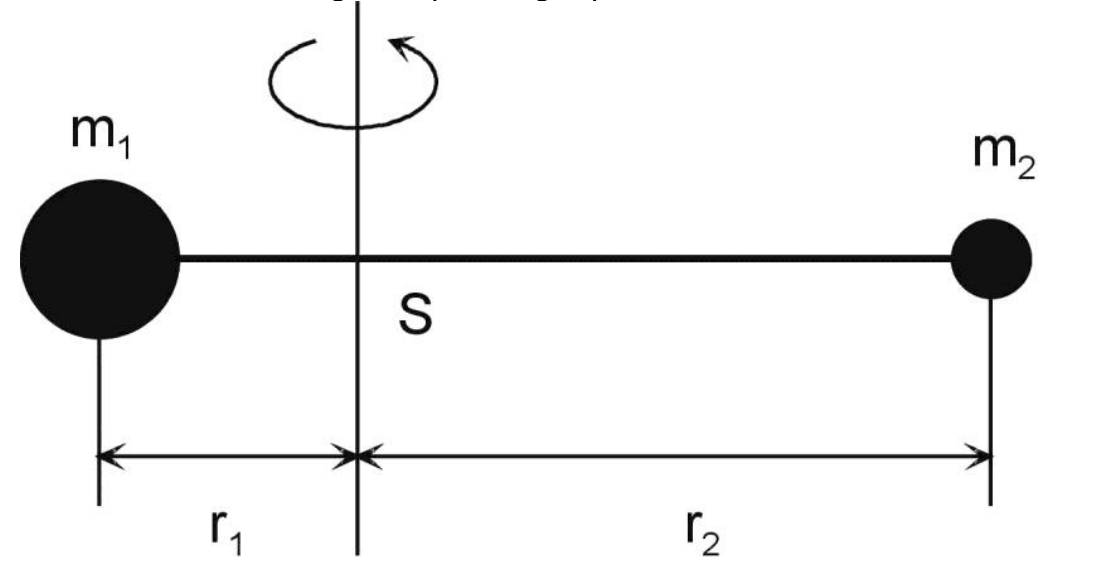
\includegraphics[width=0.55\textwidth]{hantelmodell}
  \caption{Hantelmodell eines zweiatomigen Moleküls. Die beiden Atome werden als
    punktförmige Massen $m_1$ und $m_2$ betrachtet, die auf dem festen Abstand
    $r_0$ gehalten werden. Die Rotationsachse geht durch den Massenschwerpunkt.}
  \label{fig:hantel}
\end{figure}

Die Energieeigenwerte ergeben sich aus der Schrödinger-Gleichung. Da die
Rotation potentialfrei ist ($U = 0$), lautet diese in Kugelkoordinaten für den
starren Rotator
\begin{equation}
  \frac{1}{r_0^2}\left\{
    \frac{1}{\sin\theta}\frac{\partial}{\partial\theta}
      \left(\sin\theta\,\frac{\partial\psi}{\partial\theta}\right)
    + \frac{1}{\sin^2\theta}\frac{\partial^2\psi}{\partial\phi^2}
  \right\}
  + \frac{8\pi^2\mu E}{h^2}\,\psi = 0 .
\end{equation}
Ihre Lösung liefert diskrete Energieeigenwerte
\begin{equation}
  E(J) = \frac{h^2}{8\pi^2\mu r_0^2}\,J(J+1), \qquad J = 0,1,2,\dots
  \label{eq:erot}
\end{equation}
mit der ganzzahligen Rotationsquantenzahl $J$. Da in der IR-Spektroskopie mit
Wellenzahlen gearbeitet wird und $[\wz] = [E/hc]$ gilt, fasst man die Konstanten
zur \emph{Rotationskonstante}
\begin{equation}
  B = \frac{h}{8\pi^2 c\,\mu r_0^2} = \frac{h}{8\pi^2 c\,I}
  \label{eq:B}
\end{equation}
zusammen. Der Rotationsterm $F(J) = E(J)/hc$ hat die Dimension einer Wellenzahl:
\begin{equation}
  F(J) = B\,J(J+1), \qquad J = 0,1,2,\dots
  \label{eq:FJ}
\end{equation}
Quantenmechanisch sind nur Übergänge mit der Auswahlregel
\begin{equation}
  \Delta J = \pm 1
  \label{eq:auswahlrot}
\end{equation}
erlaubt. Die zu einem Übergang $J \to J+1$ gehörende Wellenzahl beträgt somit
\begin{equation}
  \wz = F(J+1) - F(J) = 2B\,(J+1), \qquad J = 0,1,2,\dots
  \label{eq:rotlinien}
\end{equation}
Das reine Rotationsspektrum besteht daher aus äquidistanten Linien mit dem
Abstand $\wz = 2B$; es liegt im fernen Infrarot (FIR).

% ------------------------------------------------------------------
\subsection{Schwingung eines zweiatomigen Moleküls}
\label{sec:schwingung}

Im Gegensatz zur Annahme des starren Rotators sind die beiden Atome nicht durch
eine starre Stange, sondern durch Bindungskräfte verbunden. In erster Ordnung
lassen sich diese als \emph{harmonischer Oszillator} mit der Kraftkonstante $k$
nähern. Mit den Auslenkungen $x_1$ und $x_2$ aus der Ruhelage und $x = x_1 - x_2$
folgt aus den Bewegungsgleichungen die Schwingungsgleichung des harmonischen
Oszillators,
\begin{equation}
  \ddot{x} = -\frac{k}{\mu}\,x ,
\end{equation}
mit der Resonanzwellenzahl
\begin{equation}
  \wzs = \frac{1}{2\pi c}\sqrt{\frac{k}{\mu}} .
  \label{eq:nus}
\end{equation}
Die Kraftkonstante $k$ ist ein Maß für die Bindungskräfte im Molekül. Die
quantenmechanische Behandlung über die Schrödinger-Gleichung liefert die
diskreten, äquidistanten Energieeigenwerte
\begin{equation}
  E(n) = hc\,\wzs\left(n + \tfrac{1}{2}\right), \qquad n = 0,1,2,\dots
  \label{eq:eschwing}
\end{equation}
mit der Schwingungsquantenzahl $n$; $E(0) = \tfrac{1}{2}hc\,\wzs$ ist die
Nullpunktsenergie. Nach den quantenmechanischen Auswahlregeln sind nur
Dipolübergänge mit
\begin{equation}
  \Delta n = \pm 1
  \label{eq:auswahlschwing}
\end{equation}
erlaubt. Die zugehörige Übergangsenergie $E(n+1) - E(n) = hc\,\wzs$ ist
unabhängig von $n$; im reinen Schwingungsspektrum tritt also nur eine einzige
Absorptionslinie bei der Resonanzwellenzahl \wzs{} auf. Der Schwingungsterm
lautet
\begin{equation}
  G(n) = \frac{E(n)}{hc} = \wzs\left(n + \tfrac{1}{2}\right) .
  \label{eq:Gn}
\end{equation}

% ------------------------------------------------------------------
\subsection{Rotations-Schwingungsspektren}
\label{sec:rotvib}

In der Realität treten Rotation und Schwingung gleichzeitig auf. Vernachlässigt
man zunächst die Kopplung zwischen beiden, so ergibt sich die Gesamtenergie des
rotierenden Oszillators durch Addition von \eqref{eq:erot} und
\eqref{eq:eschwing},
\begin{equation}
  E(n,J) = hc\,B\,J(J+1) + hc\,\wzs\left(n + \tfrac{1}{2}\right),
  \label{eq:enJ}
\end{equation}
und für den Rotations-Schwingungsterm $T(n,J) = E(n,J)/hc$
\begin{equation}
  T(n,J) = B\,J(J+1) + \wzs\left(n + \tfrac{1}{2}\right) .
  \label{eq:TnJ}
\end{equation}
Die Auswahlregeln lauten nun
\begin{equation}
  \Delta J = \pm 1, \qquad \Delta n = 0, \pm 1 .
\end{equation}
Übergänge mit $\Delta n = 0$ liefern das reine Rotationsspektrum (FIR).
Da beim HCl die Schwingungswellenzahl \wzs{} sehr viel größer ist als die
Rotationskonstante $B$, spaltet sich die Schwingungsbande in zwei Zweige auf
(Abb.~\ref{fig:rotvib}). Man unterscheidet zwei Fälle:

\paragraph{R-Zweig ($\Delta n = 1$, $\Delta J = +1$).}
Die Differenz der Rotations-Schwingungsterme liefert
\begin{equation}
  \wz_R(J) = T(n+1,J+1) - T(n,J) = \wzs + 2B\,(J+1), \qquad J = 0,1,2,\dots
  \label{eq:rzweig}
\end{equation}

\paragraph{P-Zweig ($\Delta n = 1$, $\Delta J = -1$).}
Analog ergibt sich
\begin{equation}
  \wz_P(J) = T(n+1,J-1) - T(n,J) = \wzs - 2B\,J, \qquad J = 1,2,3,\dots
  \label{eq:pzweig}
\end{equation}
Wegen $\Delta J = -1$ existiert kein Übergang $P(0)$; der P-Zweig beginnt bei
$J = 1$.

% --- Abbildung Rotations-Schwingungsschema (Platzhalter) ---
\begin{figure}[H]
  \centering
  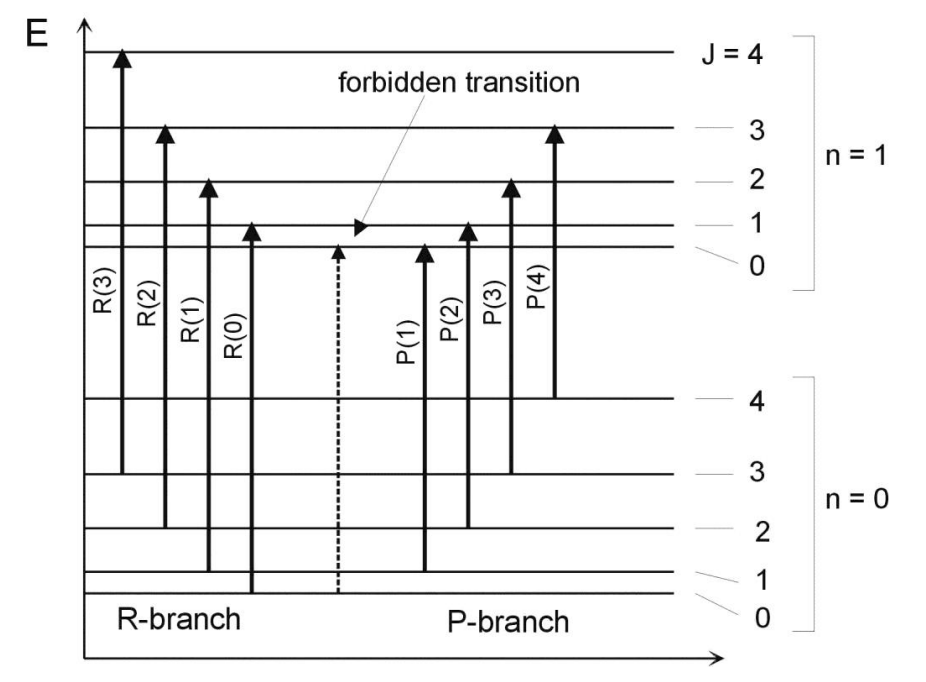
\includegraphics[width=0.6\textwidth]{rotvibschema}
  \caption{Energieniveauschema der rotierenden Schwingungszustände. Die
    Übergänge mit $\Delta J = \pm 1$ bilden für den Schwingungsmodenwechsel
    $n=0 \to n=1$ den R- und den P-Zweig aus. Der Übergang mit $\Delta J = 0$
    ist verboten.}
  \label{fig:rotvib}
\end{figure}

Da der Übergang mit $\Delta J = 0$ verboten ist, kann bei $\wz = \wzs$ keine
Linie beobachtet werden (Bandlücke). Aus den Übergangswellenzahlen lassen sich
die Kenngrößen des Moleküls bestimmen: Für die Wellenzahl des reinen
Schwingungsübergangs gilt
\begin{equation}
  \wz_R(0) + \wz_P(1) = 2\,\wzs ,
  \label{eq:nusbest}
\end{equation}
und die Rotationskonstante erhält man aus
\begin{equation}
  \wz_R(0) - \wz_P(1) = 4B .
  \label{eq:Bbest}
\end{equation}
Der Abstand zweier benachbarter Linien beträgt sowohl im P- als auch im R-Zweig
$2B$.

% ------------------------------------------------------------------
\subsection{Wechselwirkung von Rotation und Schwingung}
\label{sec:kopplung}

Die hohe Präzision des Spectrum~100 erlaubt es, die Effekte der nicht-starren
Molekülachse zu untersuchen. Am Gesamtterm $T(n,J)$ sind zwei Korrekturen
anzubringen. Zum einen vergrößert die Zentrifugalkraft der Rotation den
Atomabstand und damit das Trägheitsmoment, was zu einer Verringerung der
Rotationskonstante führt. Dieser Effekt wird durch einen quadratischen Term mit
der \emph{Dehnungskonstante} $D$ ($D \ll B$) berücksichtigt:
\begin{equation}
  F(J) = B\,J(J+1) - D\,J^2(J+1)^2 .
  \label{eq:zentrifugal}
\end{equation}
Zum anderen bewirken Anharmonizitätseffekte, dass sich der mittlere Atomabstand
zwischen den verschiedenen Schwingungszuständen ändert. Damit werden das
Trägheitsmoment und die Konstanten $B$ und $D$ von der Schwingungsquantenzahl $n$
abhängig, sodass der Rotationsterm
\begin{equation}
  F_n(J) = B_n\,J(J+1) - D_n\,J^2(J+1)^2
\end{equation}
lautet. Führt man einen laufenden Index $i$ ein ($i = -J$ für den P-Zweig,
$i = J+1$ für den R-Zweig), so lassen sich die Wellenzahlen beider Zweige unter
den Näherungen $D_n \ll B_n$ und $D_n \approx D_{n+1}$ in einer Gleichung
zusammenfassen:
\begin{equation}
  \wz(i) = \wzs + (B_1 + B_0)\,i + (B_1 - B_0)\,i^2 - 2(D_1 + D_0)\,i^3 .
  \label{eq:sammel}
\end{equation}
Der Index $i = 0$ entspricht dem verbotenen reinen Schwingungsübergang. Zur
experimentellen Bestimmung der Konstanten bildet man die erste und zweite
Differenz der Übergangswellenzahlen:
\begin{align}
  \Delta\wz(i)   &= \wz(i+1) - \wz(i)
    = 2B_1 - 2(D_1 + D_0) + 2i\bigl(B_1 - B_0 - 3(D_1 + D_0)\bigr) - 6i^2(D_1+D_0),
    \label{eq:diff1}\\
  \Delta^2\wz(i) &= \Delta\wz(i+1) - \Delta\wz(i)
    = 2(B_1 - B_0) - 12(D_1 + D_0) - 12\,i\,(D_1 + D_0) .
    \label{eq:diff2}
\end{align}
Aus dem Anstieg der Geraden \eqref{eq:diff2} erhält man $D_1 + D_0$, aus dem
Ordinatenabschnitt $B_1 - B_0$; mit \eqref{eq:diff1} können anschließend die
Einzelgrößen $B_1$ und $B_0$ bestimmt werden.

% ------------------------------------------------------------------
\subsection{Intensität des Spektrums (Bjerrum'sche Doppelbande)}
\label{sec:intensitaet}

Die Einhüllende der Absorptionslinien hat die Form einer Doppelbande: Die
Transmission durchläuft zwei Minima, die dem R- und dem P-Zweig entsprechen. Zur
Beschreibung der Intensitäten wird der Absorptionskoeffizient $\alpha$ benötigt.
Dieser ist proportional zur Übergangswahrscheinlichkeit, zur Teilchenzahl $N$ im
Ausgangszustand und zur Wellenzahl \wz{}. Unter der Annahme gleicher
Übergangswahrscheinlichkeiten für alle erlaubten Übergänge gilt
\begin{equation}
  \alpha = c_2\,N\,\wz .
  \label{eq:alpha}
\end{equation}
Im thermodynamischen Gleichgewicht ist die Zahl der Moleküle mit der Energie $E$
durch die Maxwell-Boltzmann-Verteilung gegeben:
\begin{equation}
  N(E) = \frac{\eta}{Q_r}\,e^{-E/\kB T},
  \label{eq:boltzmann}
\end{equation}
mit der Gesamtteilchenzahl $\eta$, der Zustandssumme $Q_r$, der
Boltzmann-Konstante \kB{} und der absoluten Temperatur $T$. Dabei ist zu
berücksichtigen, dass jeder Zustand mit dem Gesamtdrehimpuls $J$ $(2J+1)$-fach
entartet ist und bei Raumtemperatur nahezu alle Moleküle im
Schwingungsgrundzustand ($n = 0$) vorliegen, da die thermische Energie
$\kB T \approx \SI{26}{meV}$ deutlich kleiner ist als die Schwingungsenergie
$hc\,\wzs \approx \SI{400}{meV}$. Einsetzen von \eqref{eq:enJ} in
\eqref{eq:boltzmann} liefert für den Absorptionskoeffizienten
\begin{equation}
  \alpha = c_3\,\wz\,(2J+1)\,e^{-\frac{hc B J(J+1)}{\kB T}} .
  \label{eq:alphaJ}
\end{equation}
Mit dem Lambert'schen Gesetz ergibt sich daraus für die relative Intensität der
Absorptionslinien
\begin{equation}
  I(J) = I_0\,e^{-\alpha d}
       = I_0\exp\!\left\{ c_4\,\wz\,(2J+1)\,
         e^{-\frac{hc B J(J+1)}{\kB T}} \right\},
  \label{eq:intensitaet}
\end{equation}
wobei der Zusammenhang zwischen $J$ und \wz{} aus \eqref{eq:sammel} bekannt ist.
Über die Modellierung dieser Intensitätsverteilung lässt sich die Temperatur $T$
als freier Parameter bestimmen.

% ------------------------------------------------------------------
\subsection{Interferenzmethode zur Schichtdickenbestimmung}
\label{sec:interferenz}

Wird ein Lichtstrahl durch eine leere Küvette geführt, so wird er an den
Grenzflächen mehrfach reflektiert (Abb.~\ref{fig:kuvette}). Der transmittierte
und der mehrfach reflektierte Strahl sind kohärent und interferieren; im Spektrum
erscheint dies als periodische Modulation der Intensität. Für senkrechten Einfall
($\beta = \SI{0}{\degree}$), wie er beim näherungsweise parallelen Strahl des
Spectrum~100 vorliegt, beträgt der optische Gangunterschied zwischen dem
transmittierten und dem zweifach reflektierten Strahl
\begin{equation}
  \Delta = 2 n_0 d ,
\end{equation}
mit der Schichtdicke $d$ und dem Brechungsindex $n_0$ des Mediums.

\begin{figure}[H]
  \centering
  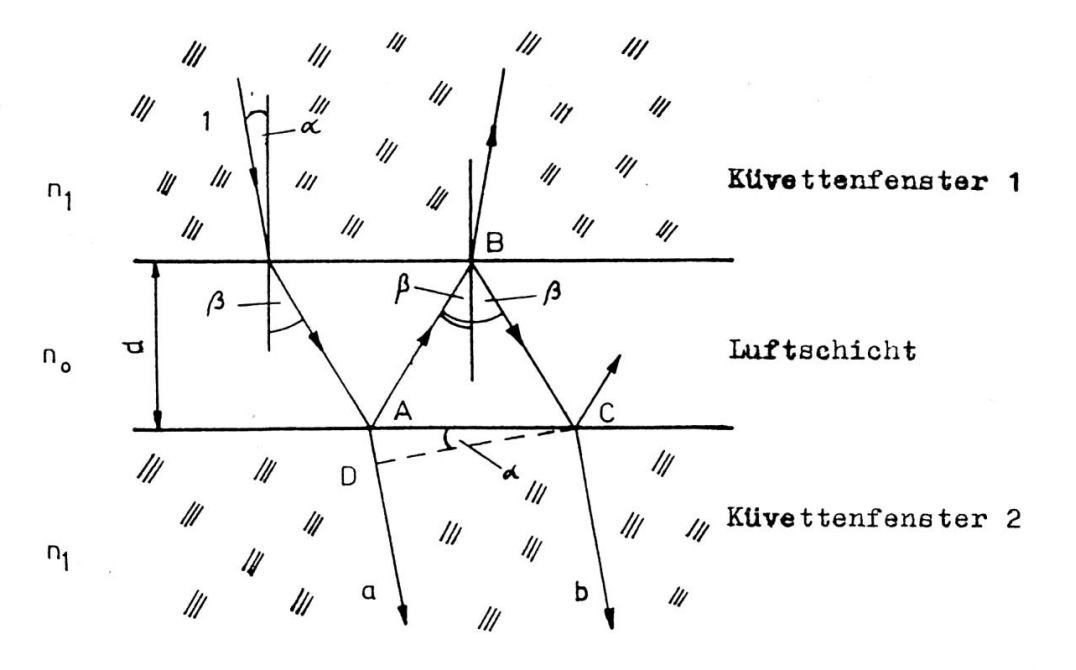
\includegraphics[width=0.6\textwidth]{kuvette}
  \caption{Strahlengang durch eine Küvette. Die durch das zweite Fenster
    austretenden Teilstrahlen $a$ und $b$ stammen aus demselben einfallenden
    Strahl~1 und sind daher kohärent. Ob sie konstruktiv oder destruktiv
    interferieren, hängt vom optischen Gangunterschied ab. Für den im Versuch
    vorliegenden senkrechten Einfall ($\beta = \SI{0}{\degree}$) vereinfacht sich
    dieser zu $\Delta = 2 n_0 d$.}
  \label{fig:kuvette}
\end{figure}

Konstruktive
Interferenz (Transmissionsmaximum) tritt auf, wenn $\Delta$ ein ganzzahliges
Vielfaches der Vakuumwellenlänge $\lambda$ ist:
\begin{equation}
  2 n_0 d = N\lambda = \frac{N}{\wz}, \qquad N = 0,1,2,\dots
\end{equation}
Betrachtet man zwei Maxima der Ordnungen $N_i$ und $N_0$ bei den Wellenzahlen
$\wz(N_i)$ und $\wz(N_0)$ und trägt die Ordnungsdifferenz $N_i - N_0$ über die
Wellenzahldifferenz auf, so ergibt sich eine Gerade mit dem Anstieg
\begin{equation}
  2 n_0 d = \frac{N_i - N_0}{\wz(N_i) - \wz(N_0)} .
  \label{eq:schichtdicke}
\end{equation}
Mit $n_0 = 1$ für Luft lässt sich die Schichtdicke $d$ aus einer linearen
Regression bestimmen.

% ------------------------------------------------------------------
\subsection{Fourier-Transformations-Infrarot-Spektroskopie}
\label{sec:ftir}

\subsubsection{Funktionsweise}

Ein FTIR-Spektrometer besteht aus einer Strahlungsquelle, einem
Interferometer (typischerweise vom Michelson-Typ) und einem Detektor. Ein
Strahlteiler spaltet das Licht der Quelle in zwei Teilstrahlen auf, die über
einen beweglichen und einen festen Spiegel geführt und anschließend wieder
vereinigt werden. Je nach optischem Wegunterschied $s = x_2 - x_1$ interferieren
die Teilstrahlen konstruktiv oder destruktiv. Für eine monochromatische Welle der
Wellenzahl \wz{} misst der Detektor die Intensität
\begin{equation}
  I(s) = I_1 + I_2 + 2\sqrt{I_1 I_2}\,\cos(2\pi\wz s) .
\end{equation}
Die als Funktion des Gangunterschieds $s$ gemessene Intensitätsverteilung $I(s)$
wird als \emph{Interferogramm} bezeichnet. Für ein kontinuierliches Spektrum
$S(\wz)$ ergibt sich das Interferogramm als Überlagerung aller
monochromatischen Beiträge,
\begin{equation}
  I(s) = 2\int_0^\infty S(\wz)\,\cos(2\pi\wz s)\,\mathrm{d}\wz .
\end{equation}
Nach Erweiterung des Integrationsbereichs auf $[-\infty,\infty]$ mittels
$S(-\wz) = S(\wz)$ folgt, dass das gesuchte Spektrum $S(\wz)$ die
Fourier-Transformierte des Interferogramms ist:
\begin{equation}
  S(\wz) = \int_{-\infty}^{\infty} I(s)\,e^{-2\pi i \wz s}\,\mathrm{d}s .
  \label{eq:ft}
\end{equation}

\subsubsection{Diskrete Fourier-Transformation, Auflösung und Zerofilling}

In der Praxis wird das Interferogramm digitalisiert und ist endlich: Es liegen
$n$ Messpunkte im konstanten Abstand $\Delta s$ vor. An die Stelle von
\eqref{eq:ft} tritt daher die diskrete Fourier-Transformation, die üblicherweise
mit dem Algorithmus der schnellen Fourier-Transformation (FFT) berechnet wird.
Aus der endlichen Weglänge folgt eine begrenzte spektrale Auflösung. Die maximal
erreichbare Wellenzahl hängt über
\begin{equation}
  \wz_{\max} \le \frac{n\,\Delta\wz}{2}
\end{equation}
mit dem Punktabstand $\Delta s$ zusammen, und der Abstand zweier Spektralpunkte
beträgt
\begin{equation}
  \Delta\wz = \frac{1}{n\,\Delta s} .
  \label{eq:aufloesung}
\end{equation}
Ein größerer Spiegelweg (mehr Datenpunkte $n$) verbessert somit das
Auflösungsvermögen. Durch \emph{Zerofilling}, d.\,h. das Anhängen von Nullen an
das Interferogramm, wird die Dichte der Spektralpunkte künstlich erhöht
(Interpolation), ohne dass echte Information hinzukommt.

\subsubsection{Leakage-Effekt und Apodisation}

Die endliche Länge des Interferogramms lässt sich mathematisch als Multiplikation
mit einer Rechteckfunktion beschreiben. Deren Fourier-Transformierte ist eine
$\mathrm{sinc}$-Funktion, die im Spektrum als eine langsam abklingende
Hintergrundschwingung um jede Spektrallinie erscheint. Dieser Effekt wird als
\emph{Leakage} bezeichnet. Multipliziert man das Interferogramm stattdessen mit
einer zu den Rändern hin sanfter abfallenden Funktion (z.\,B.
Dreieck-, Happ-Genzel- oder Blackman-Funktion), so lässt sich das Leakage unter
Einbußen bei der Maximalintensität und der Auflösung verringern. Dieser Vorgang
heißt \emph{Apodisation}; für die Auswertung ist ein Kompromiss zwischen
geringem Leakage und hohem Auflösungsvermögen zu finden. Da das gemessene
Interferogramm im Allgemeinen unsymmetrisch zum Nullpunkt aufgenommen wird,
liefert die Fourier-Transformation ein komplexwertiges Spektrum, aus dem mittels
\emph{Phasenkorrektur} (z.\,B. nach der Mertz-Methode) das reelle Spektrum
gewonnen wird.

% ==================================================================
%  4  AUSWERTUNG
% ==================================================================
\section{Auswertung}
\label{sec:auswertung}

% ------------------------------------------------------------------
\subsection{Kalibrierung der Wellenzahlskala (Aufgabe 1.1)}
\label{sec:eichung}

Zur Überprüfung der Wellenzahlskala des Spektrometers Spectrum~100 wurden
Einkanalspektren von Wasserdampf und einer Polystyrolfolie im Bereich
$\bar\nu \in [200,4000]\,\si{cm^{-1}}$ mit einem Punktabstand von
$\SI{0.125}{cm^{-1}}$ aufgenommen. Das Wasserdampfspektrum wurde ohne Probe im
Strahlengang gemessen und stellt somit das Referenz- bzw. Hintergrundspektrum
$I_0(\bar\nu)$ dar. Das Polystyrolspektrum wird daher als Transmissionsspektrum
\begin{equation}
  T(\bar\nu) = \frac{I_\mathrm{Poly}(\bar\nu)}{I_0(\bar\nu)}
  \label{eq:norm}
\end{equation}
ausgewertet. Durch diese Normierung werden sowohl der spektrale Verlauf der
Strahlungsquelle und der Gerätekomponenten als auch die scharfen
Wasserdampflinien der Umgebungsluft weitgehend herausgeteilt, sodass die breiten
Polystyrolbanden deutlicher hervortreten. Beim Wasserdampf selbst erscheinen die
Absorptionsbanden im Einkanalspektrum als lokale Minima der detektierten
Intensität.

Für jede der in der Versuchsanleitung tabellierten
Kalibrierbanden~\cite{Riede,Gupta} wurde die Lage des zugehörigen gemessenen
Minimums bestimmt, indem in einem engen Suchfenster um den Referenzwert der
tiefste Datenpunkt gesucht wurde. Die gemessenen Spektren mit den eingezeichneten
Referenz-Wellenzahlen zeigt Abb.~\ref{fig:eich_spektren}.

\begin{figure}[H]
  \centering
  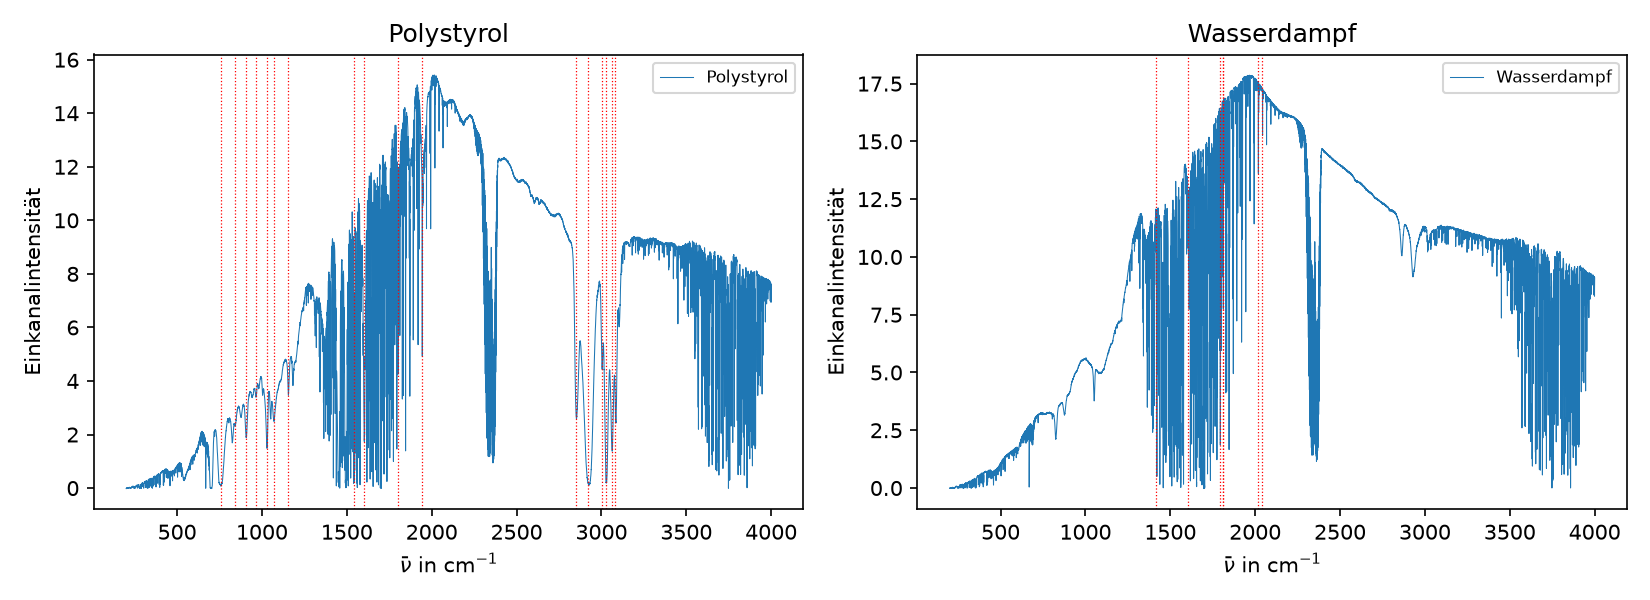
\includegraphics[width=\textwidth]{eich_spektren}
  \caption{Auf den Wasserdampf-Hintergrund normiertes Transmissionsspektrum der
    Polystyrolfolie (links) und Einkanalspektrum des Wasserdampfs (rechts). Die
    roten gepunkteten Linien markieren die zur Kalibrierung verwendeten
    theoretischen Wellenzahlen der Absorptionsbanden.}
  \label{fig:eich_spektren}
\end{figure}

Zur besseren Erkennbarkeit der einzelnen Banden zeigen die
Abbildungen~\ref{fig:eich_zoom_poly} und \ref{fig:eich_zoom_water} vergrößerte
Ausschnitte der Spektren. Die roten Punkte kennzeichnen die tiefsten Datenpunkte
der jeweiligen Absorptionsbanden, die als gemessene Bandenwellenzahlen in die
Auswertung eingehen.

\begin{figure}[H]
  \centering
  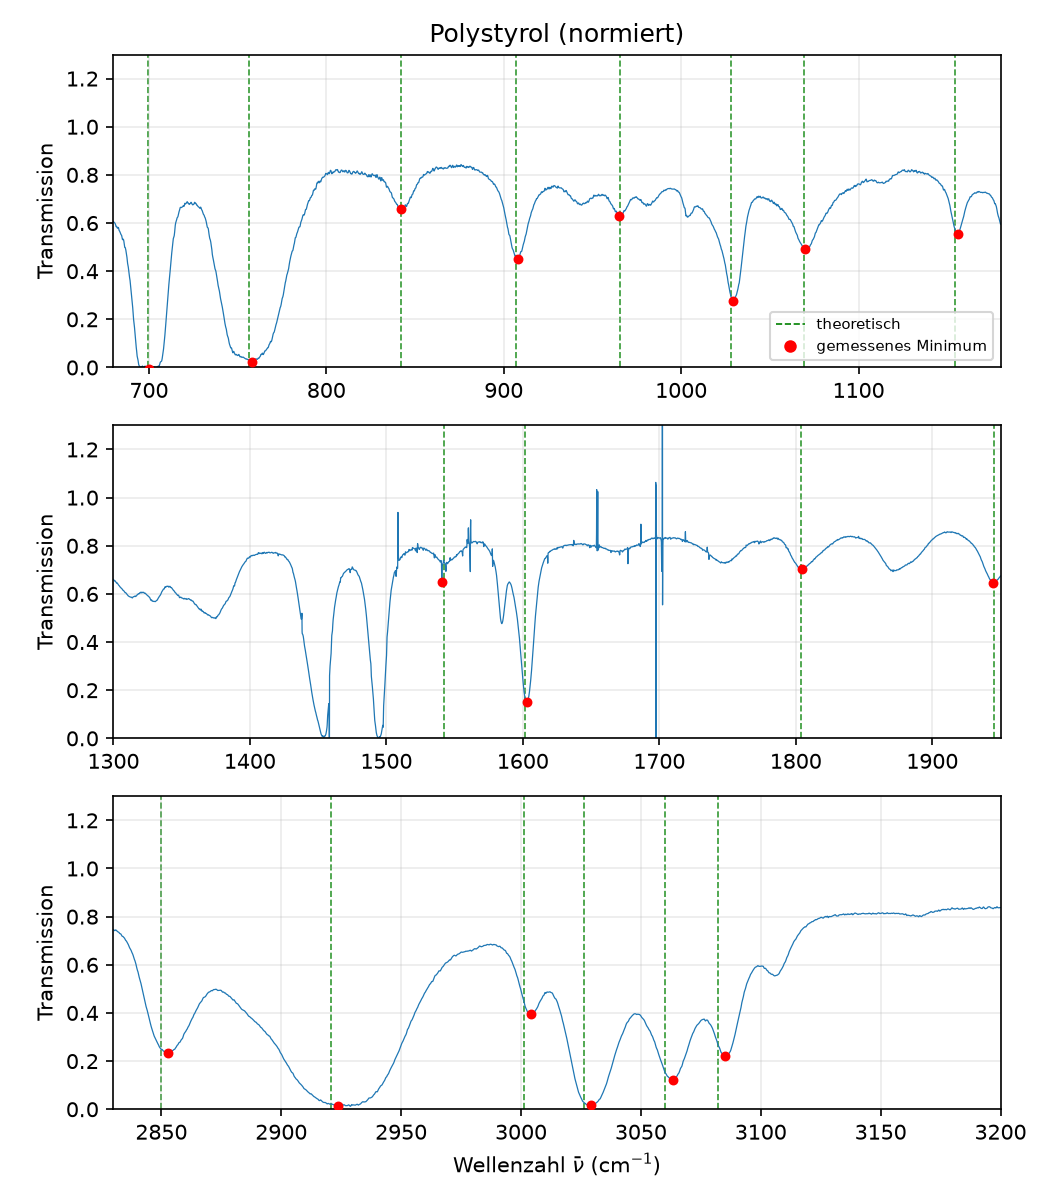
\includegraphics[width=0.72\textwidth]{eich_zoom_poly}
  \caption{Vergrößerte Ausschnitte des normierten Polystyrolspektrums. Die grünen
    gestrichelten Linien markieren die theoretischen Referenzwellenzahlen, die
    roten Punkte die zugehörigen gemessenen Bandenminima. Durch die Normierung auf
    den Hintergrund treten die Banden als klare Transmissionseinbrüche hervor;
    die vereinzelten schmalen Spikes im mittleren Fenster sind Artefakte der
    Division in Bereichen, in denen der Wasserdampf nahezu vollständig absorbiert
    ($I_0 \approx 0$).}
  \label{fig:eich_zoom_poly}
\end{figure}

\begin{figure}[H]
  \centering
  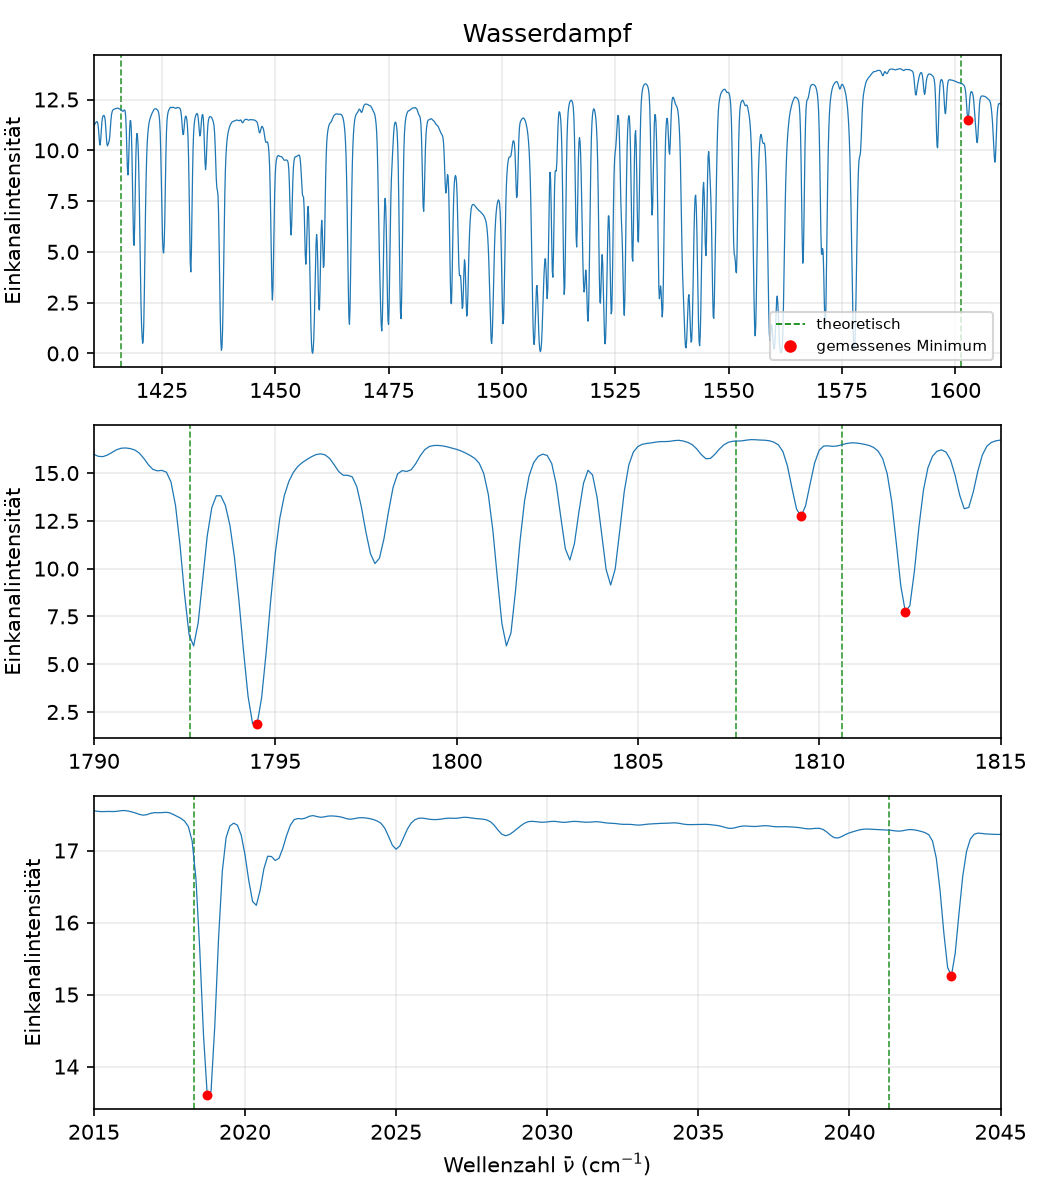
\includegraphics[width=0.72\textwidth]{eich_zoom_water}
  \caption{Vergrößerte Ausschnitte des Wasserdampfspektrums. Grüne gestrichelte
    Linien: theoretische Referenzwellenzahlen; rote Punkte: gemessene
    Bandenminima. Im Fenster um $\SI{1800}{cm^{-1}}$ ist erkennbar, dass die vier
    dicht benachbarten Referenzlinien bei der vorliegenden Auflösung nicht alle
    eindeutig getrennt werden können; markiert sind nur die verlässlich
    zuordenbaren Banden.}
  \label{fig:eich_zoom_water}
\end{figure}

Nicht alle tabellierten Banden eignen sich als Kalibrierpunkte: Beim Wasserdampf
liegen die vier Linien im Bereich um $\SI{1800}{cm^{-1}}$ so dicht beieinander,
dass sie bei der vorliegenden Auflösung nicht eindeutig getrennt werden können;
hier wurden nur die eindeutig zuordenbaren Banden verwendet. Beim Polystyrol
wurden die breiten, schwach ausgeprägten Banden bei $1368{,}5$ und
$1583{,}1\,\si{cm^{-1}}$ verworfen, da ihr Minimum auch im normierten Spektrum
nicht verlässlich der Bande zuzuordnen ist. Die Bande bei $699{,}45\,\si{cm^{-1}}$
konnte dank der Normierung, die die überlagernde Wasserdampfabsorption entfernt,
wieder aufgenommen werden. Insgesamt gingen $6$~Wasserdampf- und
$18$~Polystyrolbanden in die Auswertung ein.

Die relativen Abweichungen $(\bar\nu_\mathrm{mess}-\bar\nu_\mathrm{theo})/
\bar\nu_\mathrm{theo}$ sind in Abb.~\ref{fig:eich_abweichung} über die gemessene
Wellenzahl aufgetragen. Sie liegen betragsmäßig unterhalb von etwa
$2\cdot10^{-3}$ und streuen ohne erkennbares Muster; ein grober systematischer
Fehler ist damit auszuschließen. Der Mittelwert der relativen Abweichung beträgt
$+8{,}8\cdot10^{-4}$ (Wasserdampf) bzw.\ $+7{,}0\cdot10^{-4}$ (Polystyrol), die
gemessenen Wellenzahlen liegen also im Mittel geringfügig oberhalb der
Literaturwerte.

\begin{figure}[H]
  \centering
  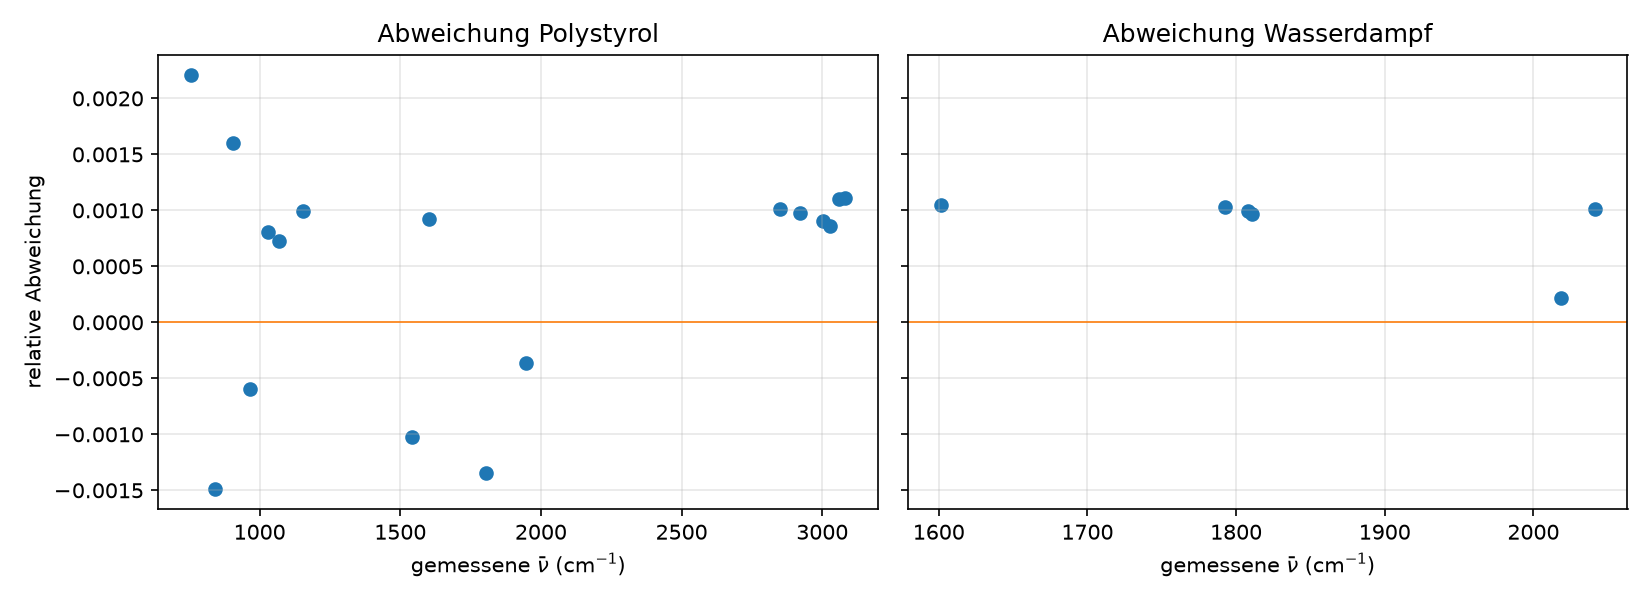
\includegraphics[width=\textwidth]{eich_abweichung}
  \caption{Relative Abweichung der gemessenen von den theoretischen
    Bandenwellenzahlen für Polystyrol (links) und Wasserdampf (rechts). Die
    waagerechte Linie kennzeichnet die Nullabweichung.}
  \label{fig:eich_abweichung}
\end{figure}

Zur Bestimmung einer möglichen Skalenkorrektur wurden die gemessenen
Bandenwellenzahlen $\bar\nu_\mathrm{mess}$ gegen die theoretischen
$\bar\nu_\mathrm{theo}$ aufgetragen und mittels linearer Regression durch
\begin{equation}
  \bar\nu_\mathrm{mess} = a\,\bar\nu_\mathrm{theo} + b
\end{equation}
angepasst (Abb.~\ref{fig:eich_regression}, aufgetragen ist die Residuendarstellung
$\bar\nu_\mathrm{mess}-\bar\nu_\mathrm{theo}$). Die Regression liefert
\begin{align}
  a &= 1{,}00103 \pm 0{,}00025, \\
  b &= (-0{,}47 \pm 0{,}49)\,\si{cm^{-1}}, \\
  R^2 &= 0{,}999999 .
\end{align}
Der Anstieg weicht mit rund $0{,}10\,\%$ nur geringfügig von $1$ ab, der
Ordinatenabschnitt ist im Rahmen seiner Unsicherheit mit $0$ verträglich. Die
Wellenzahlskala des Spektrometers ist damit innerhalb der Messgenauigkeit korrekt
kalibriert; die verbleibende Abweichung ist klein, aber statistisch signifikant
im Anstieg. Für die folgenden Auswertungen kann diese Kalibriergerade zur
Korrektur der gemessenen Wellenzahlen herangezogen werden, indem die gemessenen
Werte gemäß $\bar\nu_\mathrm{korr} = (\bar\nu_\mathrm{mess}-b)/a$ umgerechnet
werden. Wegen der Kleinheit der Korrektur ($<0{,}2\,\%$) ist ihr Einfluss auf die
weiteren Ergebnisse jedoch gering.

\begin{figure}[H]
  \centering
  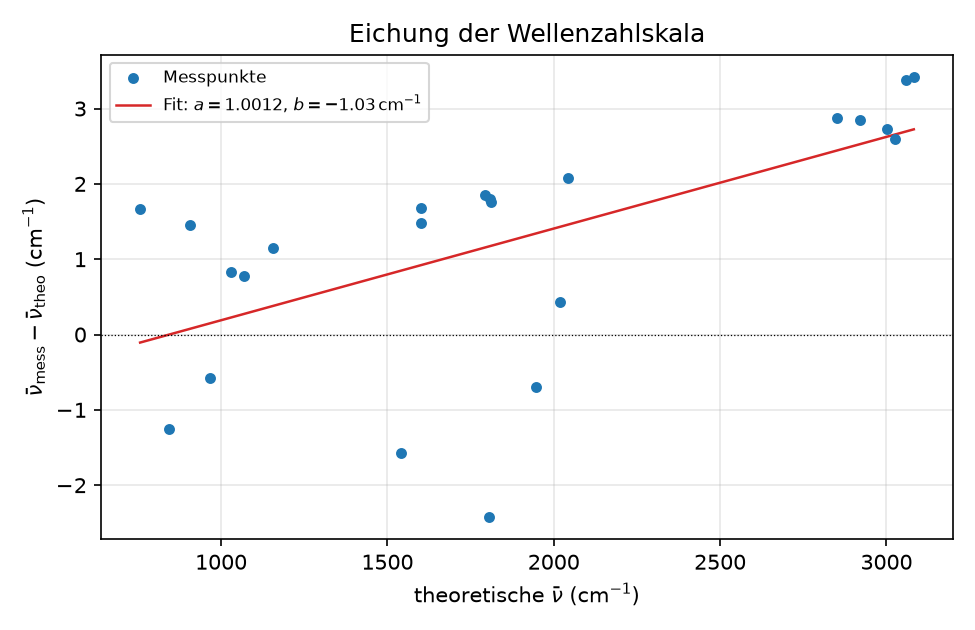
\includegraphics[width=0.7\textwidth]{eich_regression}
  \caption{Residuendarstellung der Eichung: Differenz aus gemessener und
    theoretischer Wellenzahl über der theoretischen Wellenzahl. Die rote Gerade
    entspricht der linearen Regression $\bar\nu_\mathrm{mess}=a\,
    \bar\nu_\mathrm{theo}+b$.}
  \label{fig:eich_regression}
\end{figure}

% ------------------------------------------------------------------
\subsection{Interferogramme, Fourier-Transformation und Auflösung (Aufgabe 1.2)}
\label{sec:ftir_auswertung}

Für diese Aufgabe wurden Interferogramme des Wasserdampfspektrums mit fünf
verschiedenen Spiegelbereichen des Interferometers aufgenommen. Die
Datenpunktbereiche reichen von $\pm500$ über $\pm1000$, $\pm4000$ und $\pm8000$
Punkte (jeweils symmetrisch um den Nullgangunterschied) bis zum maximalen,
einseitig verlängerten Bereich von $-8000$ bis $+32000$ Punkten. Aus jedem
Interferogramm $I(s)$ wurde das Spektrum durch eine diskrete
Fourier-Transformation (FFT) gemäß Gl.~\eqref{eq:ft} berechnet. Da die erste
Datenspalte den Punktindex und nicht direkt den optischen Weg angibt, liefert die
FFT zunächst eine Frequenzachse in Einheiten von $1/\text{Punkt}$, deren maximale
Frequenz $0{,}5$ (zwei Punkte pro Periode) beträgt. Die aufgenommenen
Interferogramme und die daraus berechneten Spektren zeigt
Abb.~\ref{fig:a2_interferogramme}.

\begin{figure}[H]
  \centering
  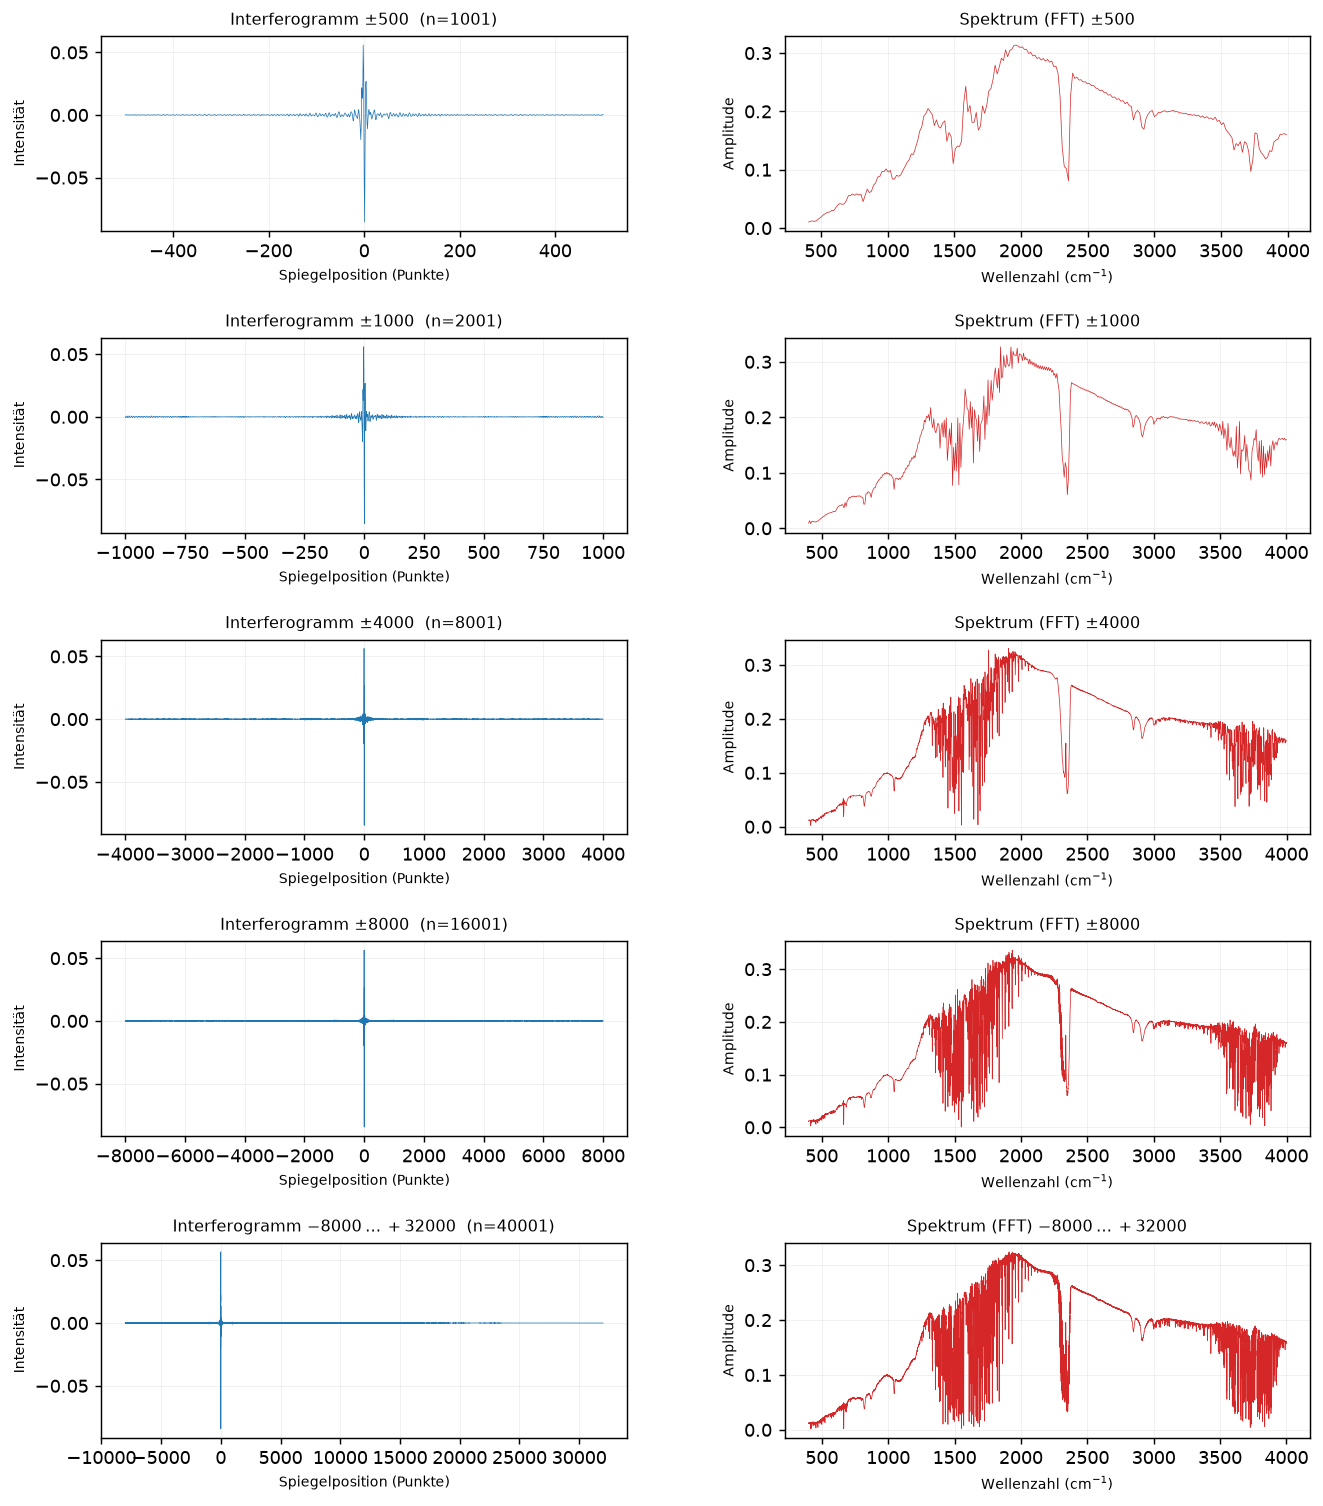
\includegraphics[width=0.86\textwidth]{a2_interferogramme}
  \caption{Aufgenommene Interferogramme (links) und die daraus per FFT berechneten
    Spektren (rechts) für die fünf Spiegelbereiche. Mit zunehmender
    Interferogrammlänge nimmt der Detailreichtum der Spektren zu. Das unterste
    Interferogramm ist einseitig verlängert ($-8000$ bis $+32000$).}
  \label{fig:a2_interferogramme}
\end{figure}

\paragraph{Schrittweite des optischen Weges.}
Zur Umrechnung der Frequenzachse in eine Wellenzahlskala wird die Schrittweite
$\Delta s$ (optischer Weg pro Datenpunkt) benötigt. Diese lässt sich aus der
Lage einer bekannten Bande im FFT-Spektrum bestimmen: Liegt ein spektrales
Merkmal bei der bekannten Wellenzahl $\bar\nu$ und der gemessenen FFT-Frequenz
$f$, so gilt $\Delta s = f/\bar\nu$. Als Referenz dient die scharfe, isolierte
Absorptionsbande des in der Umgebungsluft stets vorhandenen
Kohlendioxids bei $\bar\nu_{\mathrm{CO}_2}=\SI{2349}{cm^{-1}}$. Aus der längsten
Messung ergibt sich für ihre FFT-Frequenz $f_{\mathrm{CO}_2}=0{,}1494\,
(\text{Punkt})^{-1}$ und damit
\begin{equation}
  \Delta s = \frac{f_{\mathrm{CO}_2}}{\bar\nu_{\mathrm{CO}_2}}
           = \SI{6.36e-5}{cm} .
\end{equation}
Die daraus folgende maximal darstellbare Wellenzahl beträgt
$\bar\nu_{\max}=1/(2\Delta s)\approx\SI{7862}{cm^{-1}}$ und liegt damit oberhalb
des vom Detektor erfassten Bereichs. Die Güte dieser Kalibrierung zeigt der
Vergleich des so skalierten FFT-Spektrums mit dem korrekt kalibrierten
Referenzspektrum aus Aufgabe~1.1 in Abb.~\ref{fig:a2_kalibrierung}: Sämtliche
Wasserdampflinien und die CO$_2$-Bande fallen zusammen, was die Schrittweite
bestätigt.

\begin{figure}[H]
  \centering
  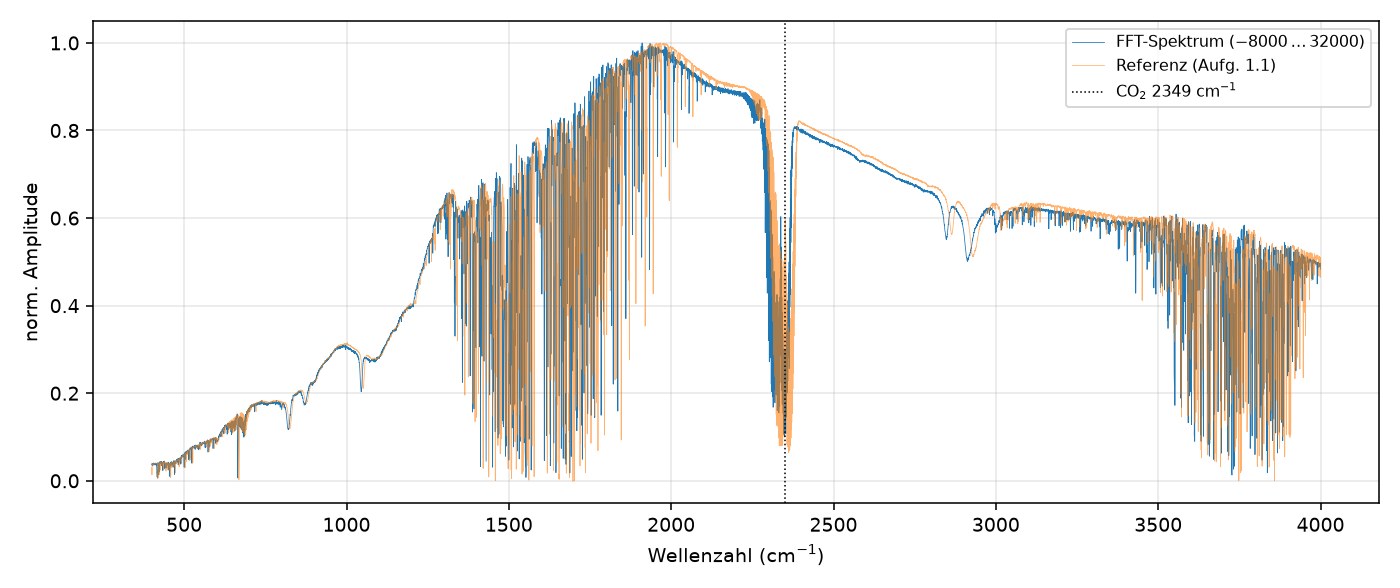
\includegraphics[width=0.85\textwidth]{a2_kalibrierung}
  \caption{Mit der aus der CO$_2$-Bande bestimmten Schrittweite kalibriertes
    FFT-Spektrum (blau) im Vergleich mit dem Referenzspektrum aus Aufgabe~1.1
    (orange). Die vollständige Übereinstimmung aller Banden bestätigt die
    ermittelte Schrittweite.}
  \label{fig:a2_kalibrierung}
\end{figure}

\paragraph{Einfluss der Interferogrammlänge.}
Abb.~\ref{fig:a2_laenge} zeigt einen Ausschnitt des Wasserdampfspektrums um
$\SI{1600}{cm^{-1}}$ für alle fünf Messungen. Die kurzen Interferogramme
($\pm500$, $\pm1000$) besitzen im dargestellten Fenster nur wenige Stützstellen
und können die dicht liegenden Rotationslinien nicht auflösen. Mit zunehmender
Länge ($\pm8000$ und die maximale Messung) werden die einzelnen Linien mit tiefen,
scharfen Einbrüchen sichtbar. Dies illustriert unmittelbar den Zusammenhang
zwischen Interferogrammlänge und spektralem Auflösungsvermögen.

\begin{figure}[H]
  \centering
  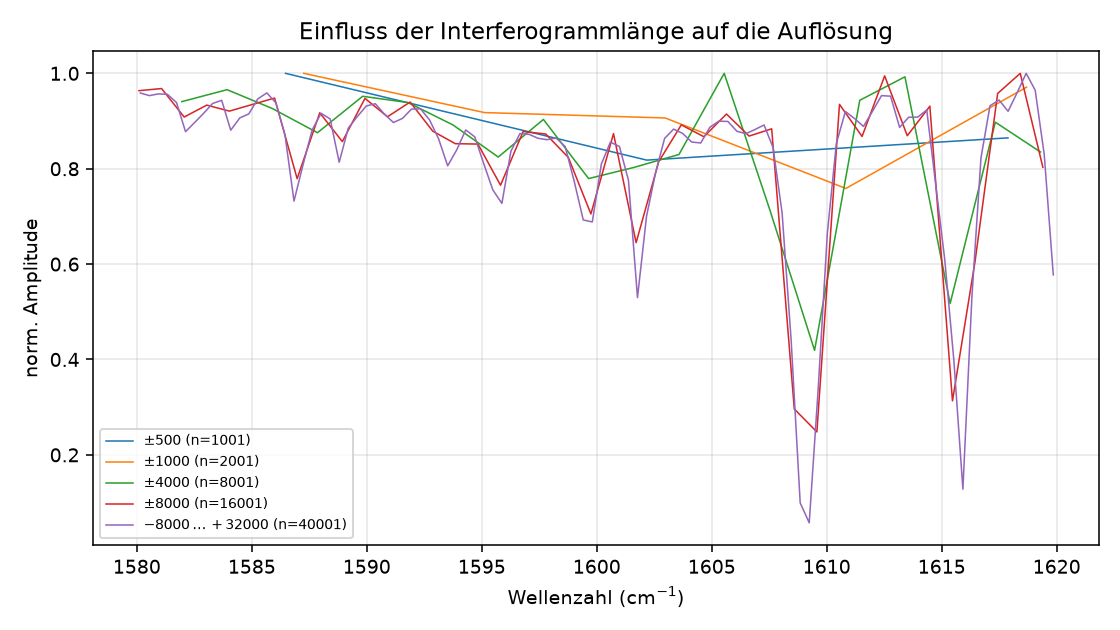
\includegraphics[width=0.72\textwidth]{a2_laenge}
  \caption{Ausschnitt des Wasserdampfspektrums um $\SI{1600}{cm^{-1}}$ für die
    fünf Interferogrammlängen. Nur die langen Interferogramme lösen die einzelnen
    Rotationslinien auf.}
  \label{fig:a2_laenge}
\end{figure}

\paragraph{Zerofilling.}
Beim Zerofilling wird das Interferogramm vor der FFT durch Anhängen von Nullen
verlängert. Abb.~\ref{fig:a2_zerofill} zeigt den Effekt für die $\pm1000$-Messung
bei Zerofilling-Faktoren von $1$ bis $8$. Die Dichte der Spektralpunkte steigt,
sodass der Kurvenverlauf glatter erscheint; die Einhüllende und damit die
tatsächliche Auflösung bleiben jedoch unverändert. Das Zerofilling wirkt somit
als reine Interpolation und fügt keine echte spektrale Information hinzu.

\begin{figure}[H]
  \centering
  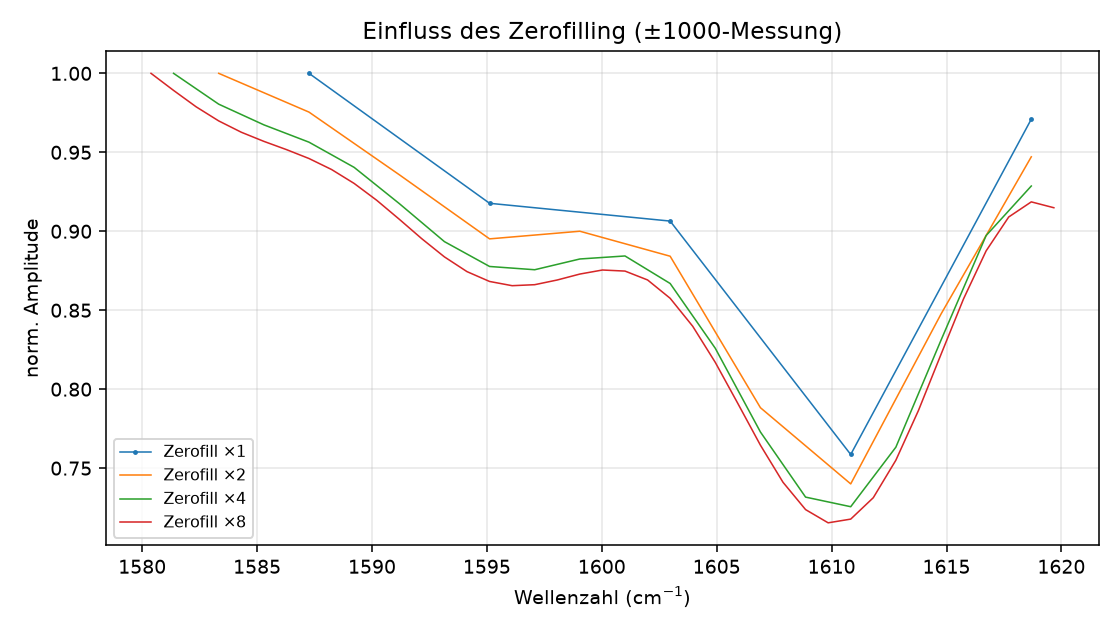
\includegraphics[width=0.72\textwidth]{a2_zerofill}
  \caption{Einfluss des Zerofilling auf das Spektrum der $\pm1000$-Messung. Höhere
    Faktoren erhöhen die Punktdichte (Interpolation), verändern aber nicht die
    Linienform bzw. die Auflösung.}
  \label{fig:a2_zerofill}
\end{figure}

\paragraph{Apodisation.}
Das abrupte Abbrechen des endlichen Interferogramms entspricht einer Multiplikation
mit einer Rechteckfunktion und führt im Spektrum zu den charakteristischen
Nebenmaxima des Leakage-Effekts (vgl.\ Abschn.~\ref{sec:ftir}).
Abb.~\ref{fig:a2_apodisation} vergleicht für die $\pm8000$-Messung die
Rechteck-, Dreieck- und Blackman-Apodisation an einer Einzellinie. Während das
Rechteckfenster deutliche Nebenschwingungen aufweist, unterdrücken das Dreieck-
und insbesondere das Blackman-Fenster diese fast vollständig -- allerdings auf
Kosten einer verbreiterten Hauptlinie und damit geringerer Auflösung. Für die
Auswertung ist folglich ein Kompromiss zwischen Leakage-Unterdrückung und
Auflösungsvermögen zu wählen.

\begin{figure}[H]
  \centering
  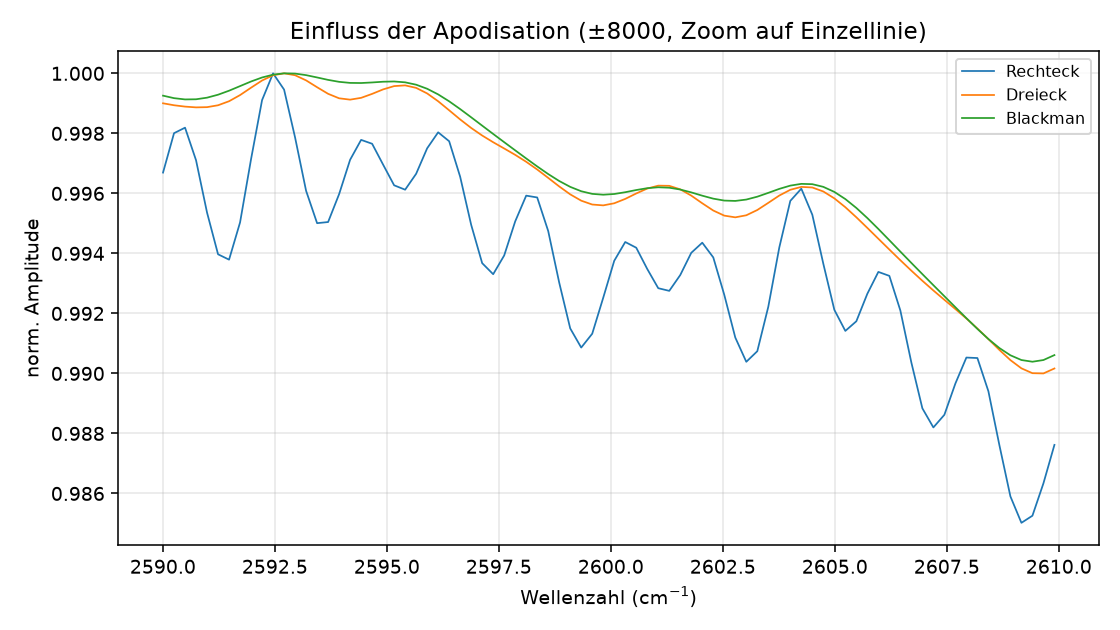
\includegraphics[width=0.72\textwidth]{a2_apodisation}
  \caption{Einfluss der Apodisationsfunktion auf eine Einzellinie
    ($\pm8000$-Messung, Zerofilling $\times4$). Das Rechteckfenster zeigt die
    stärksten Leakage-Nebenmaxima, Dreieck- und Blackman-Fenster glätten diese
    unter Verbreiterung der Hauptlinie.}
  \label{fig:a2_apodisation}
\end{figure}

\paragraph{Theoretisches Auflösungsvermögen.}
Aus der bekannten Schrittweite folgt das theoretische spektrale
Auflösungsvermögen nach Gl.~\eqref{eq:aufloesung} zu
$\Delta\bar\nu = 1/(n\,\Delta s)$, wobei $n$ die Zahl der Datenpunkte ist. Die
sich ergebenden Werte sind in Tab.~\ref{tab:a2_aufloesung} zusammengestellt und
in Abb.~\ref{fig:a2_aufloesung} als Funktion von $n$ aufgetragen.

\begin{table}[H]
  \centering
  \caption{Theoretisches Auflösungsvermögen $\Delta\bar\nu=1/(n\,\Delta s)$ für die
    fünf Interferogrammlängen ($\Delta s=\SI{6.36e-5}{cm}$).}
  \label{tab:a2_aufloesung}
  \begin{tabular}{lrr}
    \toprule
    Spiegelbereich & Punktzahl $n$ & $\Delta\bar\nu$ (cm$^{-1}$)\\
    \midrule
    $\pm500$              &  1001 & 15{,}71\\
    $\pm1000$             &  2001 &  7{,}86\\
    $\pm4000$             &  8001 &  1{,}97\\
    $\pm8000$             & 16001 &  0{,}98\\
    $-8000\dots+32000$    & 40001 &  0{,}39\\
    \bottomrule
  \end{tabular}
\end{table}

\begin{figure}[H]
  \centering
  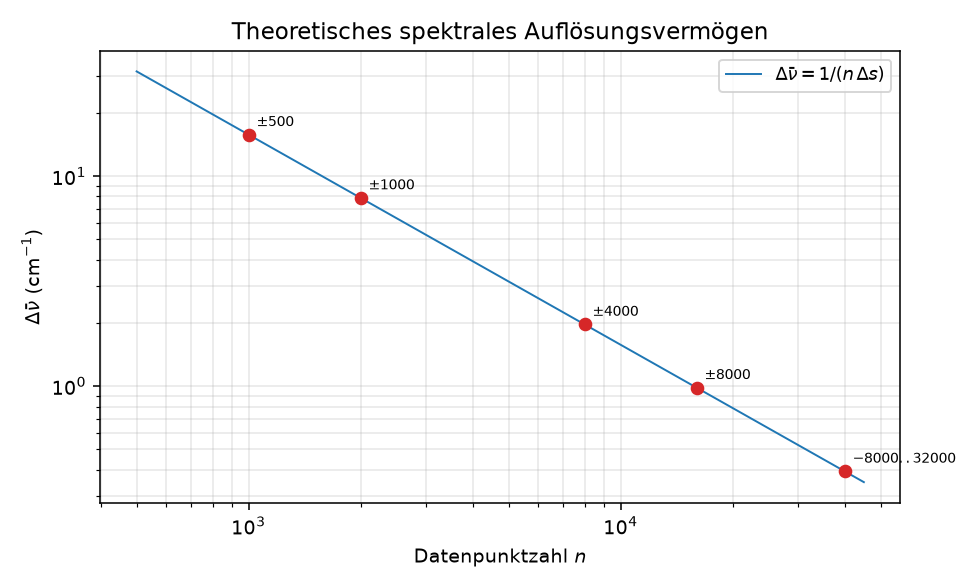
\includegraphics[width=0.62\textwidth]{a2_aufloesung}
  \caption{Theoretisches Auflösungsvermögen $\Delta\bar\nu=1/(n\,\Delta s)$ in
    Abhängigkeit von der Datenpunktzahl $n$ (doppelt-logarithmisch). Die
    Messpunkte liegen auf der theoretischen Kurve.}
  \label{fig:a2_aufloesung}
\end{figure}

Die längste Messung erreicht ein Auflösungsvermögen von etwa
$\Delta\bar\nu\approx\SI{0.4}{cm^{-1}}$, das für die Auflösung der
Rotations-Schwingungslinien des HCl (Aufgabe~1.5) ausreichend ist. Die kurzen
Interferogramme liefern mit $\Delta\bar\nu\gtrsim\SI{8}{cm^{-1}}$ hingegen nur
grob aufgelöste Spektren.

% ------------------------------------------------------------------
\subsection{Sperrverhalten von Glas- und NaCl-Filter (Aufgabe 1.3)}
\label{sec:sperrfilter}

Zur Charakterisierung des Sperrverhaltens wurden Einkanalspektren einer Glasplatte
und eines NaCl-Kristalls im Bereich $\bar\nu \in [100,6000]\,\si{cm^{-1}}$
aufgenommen. Als Referenz $I_0$ dient das ohne Probe gemessene Spektrum
(vgl.\ Aufgabe~1.1), das im Überlappungsbereich $[200,4000]\,\si{cm^{-1}}$
vorliegt. Das Transmissionsvermögen ergibt sich als $I/I_0$ nach
Gl.~\eqref{eq:norm}. Abb.~\ref{fig:a3_uebersicht} zeigt die drei Einkanalspektren
im direkten Vergleich.

\begin{figure}[H]
  \centering
  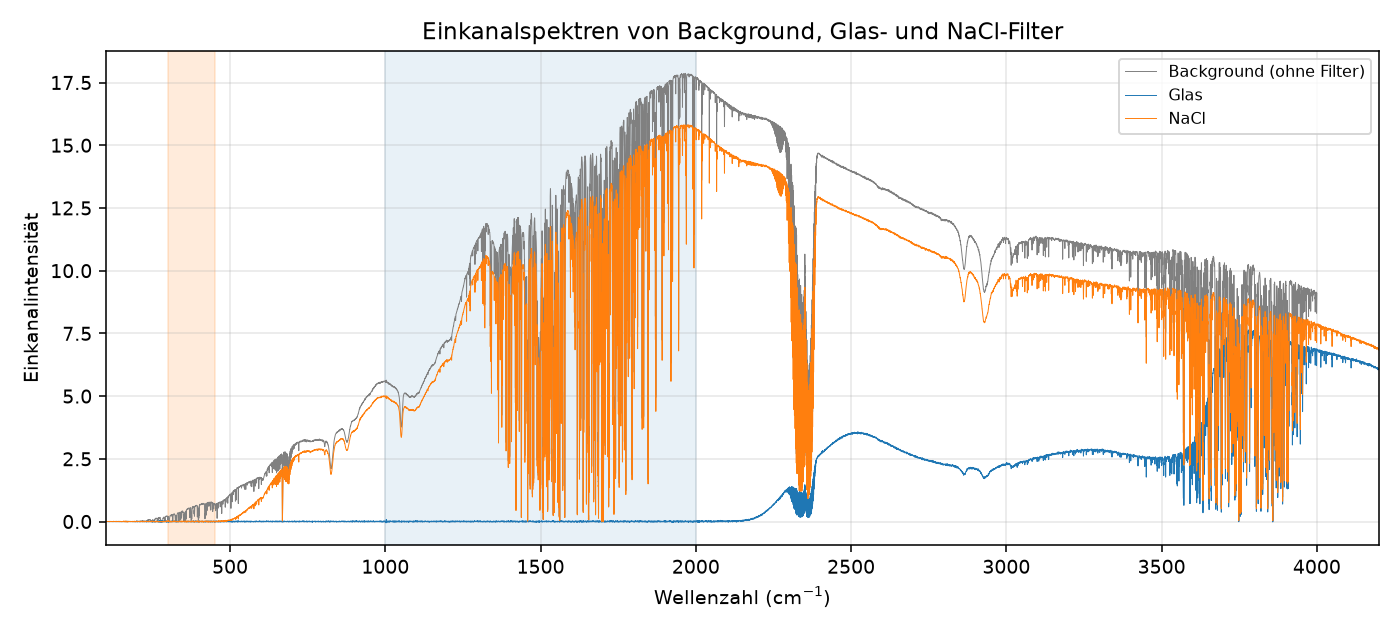
\includegraphics[width=0.9\textwidth]{a3_uebersicht}
  \caption{Einkanalspektren des Hintergrunds (grau) sowie des Glas- (blau) und
    des NaCl-Filters (orange). Farbig hinterlegt sind die zur quantitativen
    Auswertung verwendeten Sperrbereiche.}
  \label{fig:a3_uebersicht}
\end{figure}

\paragraph{Glasfilter.}
Das Transmissionsspektrum des Glases (Abb.~\ref{fig:a3_glas}) zeigt, dass Glas im
mittleren Infrarot bis etwa $\SI{2200}{cm^{-1}}$ nahezu vollständig undurchlässig
ist. Erst oberhalb steigt die Transmission an und erreicht ab etwa
$\SI{3500}{cm^{-1}}$ Werte von rund $\SI{75}{\percent}$. Im gut definierten
Sperrbereich $[1000,2000]\,\si{cm^{-1}}$, in dem die Referenzintensität hoch ist,
beträgt das Transmissionsvermögen
\begin{equation}
  \left(\frac{I}{I_0}\right)_\mathrm{Glas} = (0{,}03 \pm 0{,}27)\,\si{\percent} ,
\end{equation}
das Signal ist dort also im Rahmen des Rauschens mit null verträglich. Glas wirkt
im mittleren Infrarot damit als praktisch vollständiger Sperrfilter.

\begin{figure}[H]
  \centering
  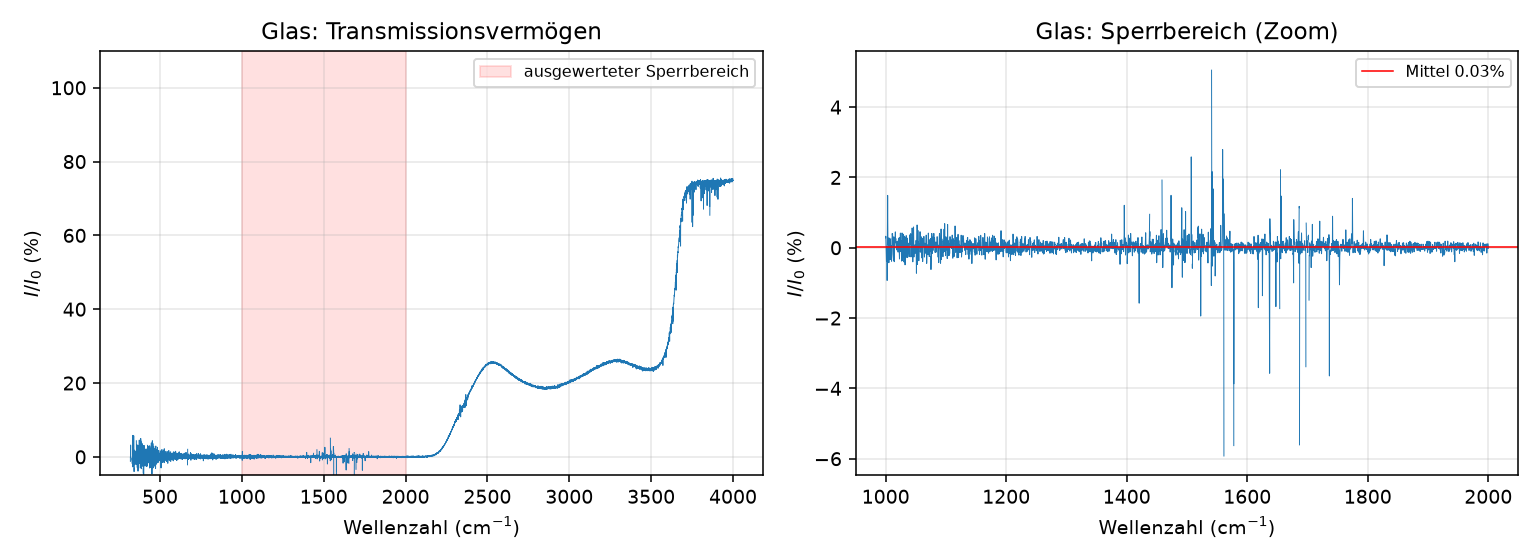
\includegraphics[width=\textwidth]{a3_glas}
  \caption{Transmissionsvermögen $I/I_0$ des Glasfilters (links) und Ausschnitt
    des Sperrbereichs (rechts). Im Sperrbereich streut das Signal um null; die
    rote Linie kennzeichnet den Mittelwert.}
  \label{fig:a3_glas}
\end{figure}

\paragraph{NaCl-Filter.}
Natriumchlorid ist im mittleren Infrarot ein Standard-Fenstermaterial. Das
gemessene Transmissionsspektrum (Abb.~\ref{fig:a3_nacl}) bestätigt dies: Oberhalb
einer Durchlasskante bei etwa $\SI{550}{cm^{-1}}$ liegt die Transmission auf einem
Plateau von rund $\SI{88}{\percent}$ und bleibt über den gesamten MIR-Bereich
hoch. Erst unterhalb von etwa $\SI{500}{cm^{-1}}$ setzt die Absorption
(Gitterschwingungen) ein. Im Sperrbereich $[300,450]\,\si{cm^{-1}}$ beträgt das
Transmissionsvermögen
\begin{equation}
  \left(\frac{I}{I_0}\right)_\mathrm{NaCl} = (0{,}35 \pm 1{,}79)\,\si{\percent} ,
\end{equation}
im Durchlassbereich $[1000,3000]\,\si{cm^{-1}}$ dagegen $(88{,}3 \pm
0{,}7)\,\si{\percent}$. Die vergleichsweise große Streuung im Sperrbereich ist
darauf zurückzuführen, dass dort auch die Referenzintensität $I_0$ klein ist,
sodass sich das Rauschen bei der Division stark auswirkt.

\begin{figure}[H]
  \centering
  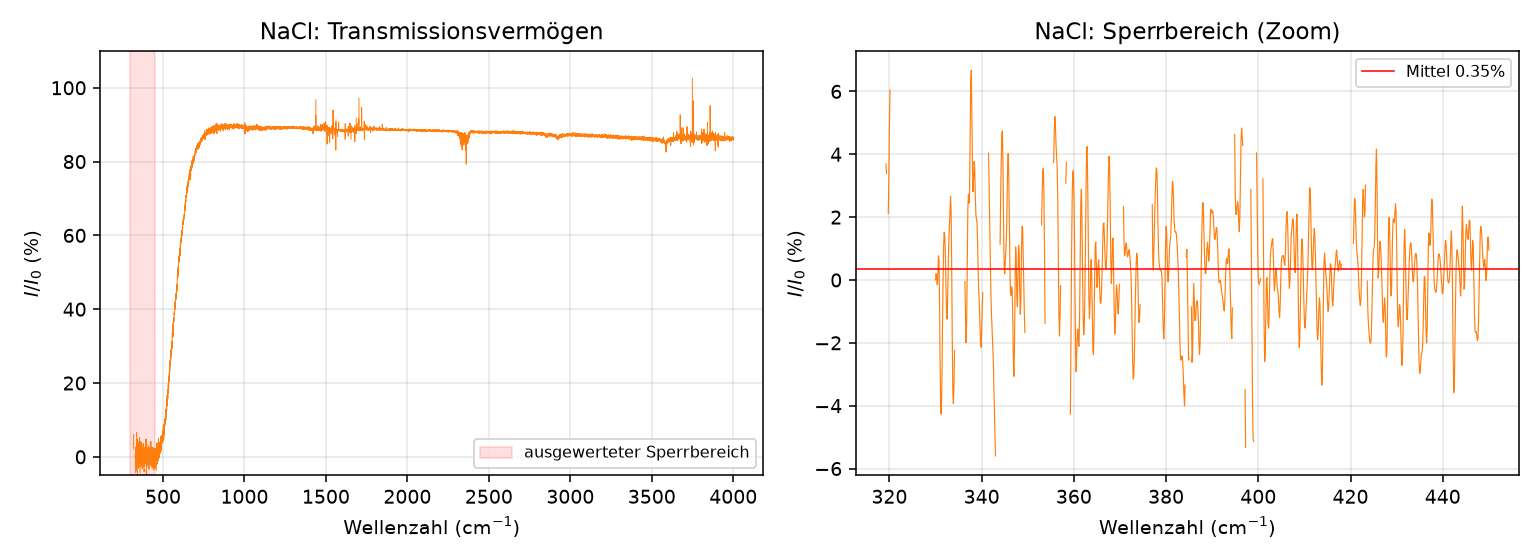
\includegraphics[width=\textwidth]{a3_nacl}
  \caption{Transmissionsvermögen $I/I_0$ des NaCl-Filters (links) und Ausschnitt
    des Sperrbereichs (rechts). Oberhalb der Durchlasskante bei $\approx
    \SI{550}{cm^{-1}}$ ist NaCl nahezu transparent.}
  \label{fig:a3_nacl}
\end{figure}

Zusammenfassend blockiert das Glas das gesamte mittlere Infrarot bis etwa
$\SI{2200}{cm^{-1}}$, während NaCl in diesem Bereich transparent ist und lediglich
das ferne Infrarot unterhalb $\SI{500}{cm^{-1}}$ sperrt. Beide zeigen im jeweiligen
Sperrbereich ein Transmissionsvermögen von deutlich unter $\SI{1}{\percent}$.

% ------------------------------------------------------------------
\subsection{Spaltbreite einer Küvette (Aufgabe 1.4)}
\label{sec:kuvette}

Beim Durchgang durch eine leere Küvette interferiert der transmittierte mit dem
mehrfach reflektierten Strahl, was im Spektrum eine periodische Modulation
(Etalon-Interferenzen) erzeugt. Aus deren Periode lässt sich nach
Gl.~\eqref{eq:schichtdicke} die Spaltbreite $d$ bestimmen. Es wurden zwei leere
Küvetten vermessen; da beide klare, gut auswertbare Interferenzmuster zeigen,
werden sie hier ausgewertet und die Ergebnisse als Konsistenzprüfung verglichen.
Zur Berechnung des Transmissionsvermögens wurden die Einkanalspektren wie zuvor
auf das Hintergrundspektrum normiert. Abb.~\ref{fig:a4_uebersicht} zeigt die
resultierenden periodischen Interferenzmuster beider Küvetten.

\begin{figure}[H]
  \centering
  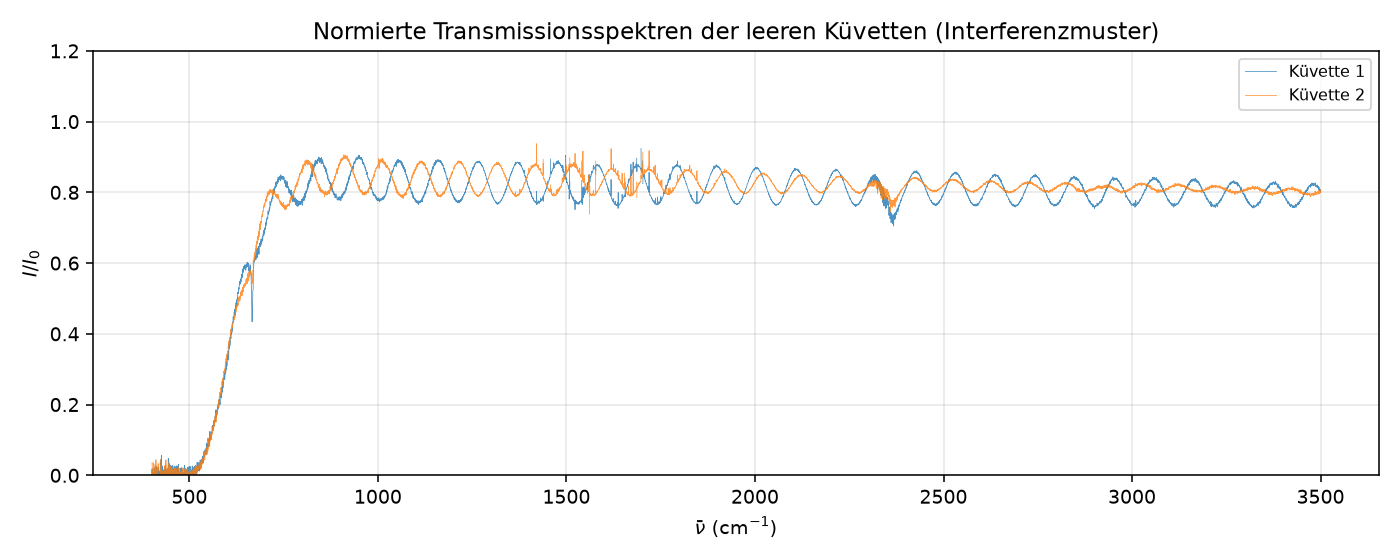
\includegraphics[width=0.92\textwidth]{a4_uebersicht}
  \caption{Auf den Hintergrund normierte Transmissionsspektren der beiden leeren
    Küvetten. Die periodische Modulation ist das für die Auswertung genutzte
    Etalon-Interferenzmuster. Beide Küvetten weisen eine sehr ähnliche Periode
    (und damit Spaltbreite) auf.}
  \label{fig:a4_uebersicht}
\end{figure}

Zur Bestimmung der Fringe-Periode wurde zunächst der (langsam veränderliche)
spektrale Untergrund abgezogen und das verbleibende Signal mit einem Bandpass um
die dominante, per Fourier-Transformation ermittelte Modulationsfrequenz
gefiltert. Anschließend wurden die Maxima des Interferenzmusters detektiert und
mit fortlaufenden Ordnungen $N$ versehen. Nach Gl.~\eqref{eq:schichtdicke} liefert
die Auftragung der Ordnung $N$ über die Wellenzahl $\bar\nu$ eine Gerade mit dem
Anstieg $2d$ (mit $n_0=1$ für Luft). Die lineare Regression
(Abb.~\ref{fig:a4_interferenz}) ergibt
\begin{align}
  d_1 &= (47{,}5 \pm 1{,}0)\,\si{\micro\metre} \quad \text{(Küvette 1)},\\
  d_2 &= (49{,}8 \pm 1{,}0)\,\si{\micro\metre} \quad \text{(Küvette 2)},
\end{align}
jeweils mit einem Bestimmtheitsmaß $R^2 > 0{,}9999$. Als Unsicherheit ist nicht
der (unrealistisch kleine) rein statistische Regressionsfehler angegeben, sondern
die Abweichung zwischen der Peak- und einer unabhängigen
Fourier-Analyse des Interferenzmusters, die die tatsächliche Methodengenauigkeit
besser widerspiegelt.

\begin{figure}[H]
  \centering
  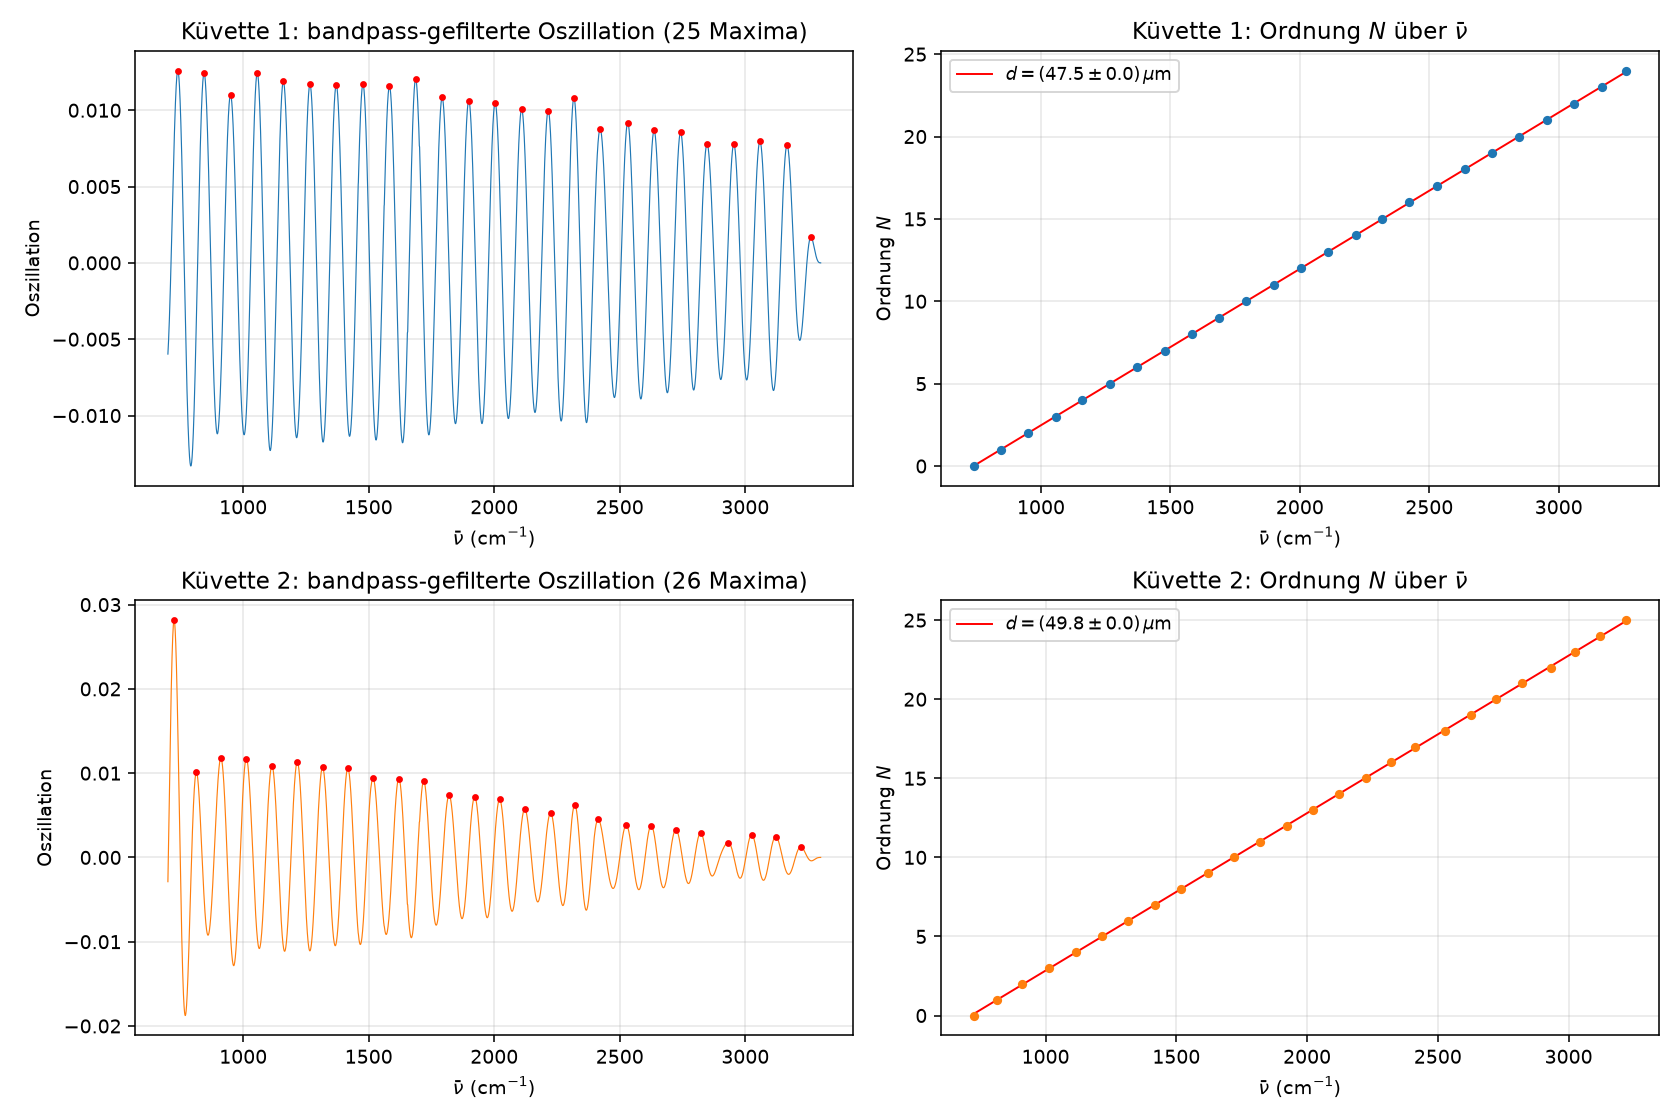
\includegraphics[width=\textwidth]{a4_interferenz}
  \caption{Auswertung der Interferenzmethode für beide Küvetten. Links: das
    bandpass-gefilterte Interferenzmuster mit den detektierten Maxima (rot).
    Rechts: Ordnung $N$ über der Wellenzahl $\bar\nu$ mit linearer Regression; der
    Anstieg entspricht $2d$.}
  \label{fig:a4_interferenz}
\end{figure}

Beide Küvetten liefern innerhalb der Fehlergrenzen übereinstimmende Spaltbreiten
von rund $\SI{48}{\micro\metre}$ bzw.\ $\SI{50}{\micro\metre}$, was die Zuverlässigkeit
der Interferenzmethode belegt. Die Werte liegen in derselben Größenordnung wie die
in vergleichbaren Messungen bestimmten Schichtdicken~\cite{Geschke}.

% ------------------------------------------------------------------
\subsection{Rotations-Schwingungsspektrum von HCl (Aufgabe 1.5)}
\label{sec:hcl}

\paragraph{Vorbemerkung.} Die Aufnahme des HCl-Spektrums war am Versuchstag vor
Ort nicht möglich. Die im Folgenden ausgewerteten Daten (Spektrum der
HCl-Gasküvette sowie zugehöriges Hintergrundspektrum) wurden uns daher vom
Versuchsleiter zur Verfügung gestellt.

Zur Auswertung wurde das Einkanalspektrum der HCl-Küvette auf das mitgelieferte
Hintergrundspektrum normiert. Das resultierende Transmissionsspektrum zeigt im
Bereich $\bar\nu \in [2700,3050]\,\si{cm^{-1}}$ die für ein zweiatomiges Molekül
charakteristische Rotations-Schwingungsbande mit einem P- und einem R-Zweig, die
durch die verbotene reine Schwingungslinie ($\Delta J = 0$) bei etwa
$\SI{2887}{cm^{-1}}$ getrennt sind (Abb.~\ref{fig:a5_zuordnung}, oben). Jede Linie
ist zudem in ein Dublett aufgespalten, das von den beiden Chlorisotopen
$^{35}\mathrm{Cl}$ und $^{37}\mathrm{Cl}$ herrührt. Da die reduzierte Masse des
leichteren Isotopologs $\mathrm{H}^{35}\mathrm{Cl}$ kleiner ist, liegen dessen
Linien bei geringfügig höheren Wellenzahlen; die jeweils höhere (und intensivere)
Linie eines Dubletts wird daher $^{35}\mathrm{Cl}$ zugeordnet.

\begin{figure}[H]
  \centering
  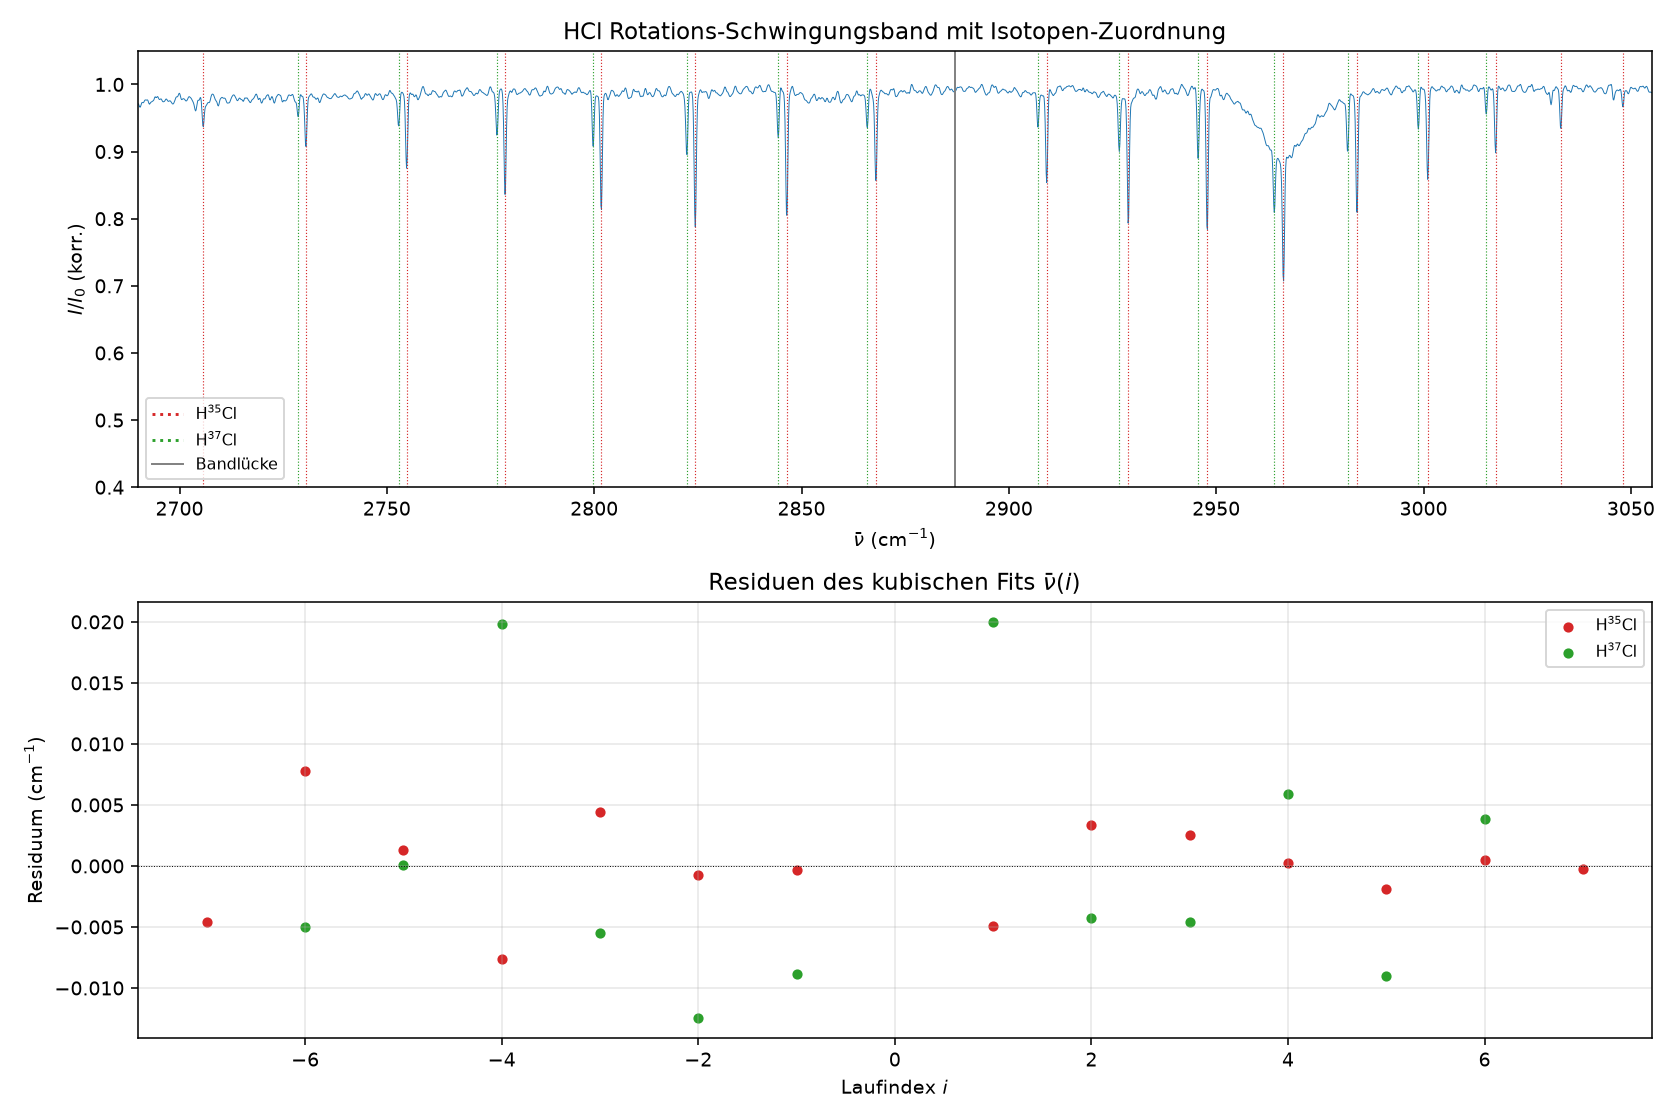
\includegraphics[width=\textwidth]{a5_zuordnung}
  \caption{Oben: normiertes und untergrundkorrigiertes Transmissionsspektrum von
    HCl mit der Zuordnung der Linien zu $\mathrm{H}^{35}\mathrm{Cl}$ (rot) und
    $\mathrm{H}^{37}\mathrm{Cl}$ (grün) sowie der Bandlücke. Unten: Residuen des
    kubischen Fits $\bar\nu(i)$ nach Gl.~\eqref{eq:sammel} für beide Isotope.}
  \label{fig:a5_zuordnung}
\end{figure}

\paragraph{Bestimmung der Molekülkonstanten.}
Die Linienpositionen wurden für jedes Isotop getrennt bestimmt und mit dem
laufenden Index $i$ versehen ($i=J+1$ für den R-Zweig, $i=-J$ für den P-Zweig).
Ein kubischer Fit gemäß Gl.~\eqref{eq:sammel},
\begin{equation*}
  \bar\nu(i) = \bar\nu_S + (B_1+B_0)\,i + (B_1-B_0)\,i^2 - 2(D_1+D_0)\,i^3 ,
\end{equation*}
liefert unmittelbar die Bandmitte $\bar\nu_S$, die Rotationskonstanten $B_0$ und
$B_1$ sowie die Dehnungskonstante $D$. Die Residuen dieses Fits liegen für beide
Isotope unterhalb von $\SI{0.02}{cm^{-1}}$ (Abb.~\ref{fig:a5_zuordnung}, unten)
und zeigen kein systematisches Muster. Aus $B_0$ folgt das Trägheitsmoment
$I = h/(8\pi^2 c\,B_0)$, daraus der Kernabstand $r_0=\sqrt{I/\mu}$ und aus
$\bar\nu_S$ die Kraftkonstante $k = (2\pi c\,\bar\nu_S)^2\,\mu$. Die Ergebnisse
sind in Tab.~\ref{tab:a5} zusammengefasst.

\begin{table}[H]
  \centering
  \caption{Aus dem Rotations-Schwingungsspektrum bestimmte Molekülkonstanten für
    die beiden Isotopologe, im Vergleich mit Literaturwerten~\cite{Rinsland,Demtroeder}.}
  \label{tab:a5}
  \begin{tabular}{lccc}
    \toprule
    Größe & $\mathrm{H}^{35}\mathrm{Cl}$ & $\mathrm{H}^{37}\mathrm{Cl}$ & Literatur ($^{35}$)\\
    \midrule
    $\bar\nu_S$ (cm$^{-1}$)       & $2888{,}8 \pm 0{,}9$ & $2886{,}7 \pm 0{,}9$ & $2885{,}9$\\
    $B_0$ (cm$^{-1}$)             & $10{,}450 \pm 0{,}022$ & $10{,}437 \pm 0{,}027$ & $10{,}44$\\
    $B_1$ (cm$^{-1}$)             & $10{,}146 \pm 0{,}022$ & $10{,}133 \pm 0{,}027$ & $10{,}14$\\
    $D_1{+}D_0$ ($10^{-3}\,$cm$^{-1}$) & $1{,}05 \pm 0{,}58$ & $1{,}09 \pm 0{,}98$ & $1{,}06$\\
    $I$ ($10^{-47}\,$kg\,m$^2$)   & $2{,}679 \pm 0{,}006$ & $2{,}682 \pm 0{,}007$ & $2{,}64$\\
    $r_0$ (pm)                    & $128{,}3 \pm 0{,}1$ & $128{,}3 \pm 0{,}2$ & $127{,}5$\\
    $k$ (N/m)                     & $481{,}7 \pm 0{,}3$ & $481{,}7 \pm 0{,}3$ & $480$\\
    \bottomrule
  \end{tabular}
\end{table}

Sämtliche Werte stimmen sehr gut mit den Literaturwerten überein. Die
schwingungsabhängige Rotationskonstante zeigt mit $B_1 < B_0$ das erwartete
Verhalten: Im angeregten Schwingungszustand ist der mittlere Kernabstand größer,
das Trägheitsmoment somit größer und die Rotationskonstante kleiner.

\paragraph{Isotopeneffekt.}
Die Verhältnisse der Konstanten beider Isotopologe bestätigen die theoretische
Massenabhängigkeit. Wegen $\bar\nu_S \propto \mu^{-1/2}$ und $B \propto \mu^{-1}$
erwartet man
\begin{align*}
  \frac{\bar\nu_S(^{35})}{\bar\nu_S(^{37})} &= \sqrt{\frac{\mu_{37}}{\mu_{35}}} = 1{,}00076,
  & \frac{B_0(^{35})}{B_0(^{37})} &= \frac{\mu_{37}}{\mu_{35}} = 1{,}00152 .
\end{align*}
Gemessen wurden $1{,}00073\pm0{,}00043$ bzw.\ $1{,}0013\pm0{,}0033$, beide
innerhalb ihrer Unsicherheiten in Übereinstimmung mit der Theorie (vgl.\
Abschn.~\ref{sec:fehler}).

\paragraph{Häufigkeitsverhältnis der Isotope.}
Nach dem Lambert-Beer'schen Gesetz ist die Absorbanz $A=-\ln(I/I_0)$ proportional
zur Teilchenzahl des jeweiligen Isotopologs. Aus dem Verhältnis der integrierten
Absorbanz zusammengehöriger Dublett-Linien ergibt sich das Häufigkeitsverhältnis
\begin{equation}
  \frac{N_{35}}{N_{37}} = 1{,}96 \pm 0{,}08 .
\end{equation}
Der Wert liegt unter dem natürlichen Häufigkeitsverhältnis von
$N_{35}/N_{37} \approx 3{,}13$~\cite{Rinsland}. Diese Abweichung ist auf eine
teilweise Sättigung der intensiveren $^{35}\mathrm{Cl}$-Linien zurückzuführen,
deren Absorbanz dadurch unterschätzt wird; ein vergleichbarer Wert wird auch in
anderen Auswertungen dieses Versuchs beobachtet.

% ------------------------------------------------------------------
\subsection{Intensitätsmodellierung und Temperaturbestimmung (Aufgabe 1.6)}
\label{sec:intensitaet_aufg}

Abschließend werden die Intensitäten der Absorptionslinien im P-Zweig modelliert.
Nach Gl.~\eqref{eq:alphaJ} ist der Absorptionskoeffizient und damit -- über das
Lambert'sche Gesetz -- die Absorbanz $A=-\ln(I/I_0)$ proportional zu
\begin{equation}
  A(J) \propto \bar\nu\,(2J+1)\,
        \exp\!\left(-\frac{hc\,B_0\,J(J+1)}{\kB T}\right) .
  \label{eq:intmodell}
\end{equation}
Der Faktor $(2J+1)$ beschreibt die Entartung der Rotationsniveaus, der
Boltzmann-Faktor deren thermische Besetzung. Das Produkt beider Terme führt zu
einem Intensitätsmaximum bei einem mittleren $J$, dessen Lage von der Temperatur
abhängt. Für die Auswertung wurden die Absorbanzen der P-Zweig-Linien des
Isotopologs $\mathrm{H}^{35}\mathrm{Cl}$ aus dem Transmissionsspektrum bestimmt und
den Rotationsquantenzahlen $J=1,\dots,8$ zugeordnet. Mit der in Aufgabe~1.5
bestimmten Rotationskonstante $B_0$ wurde Gl.~\eqref{eq:intmodell} mit der
Temperatur $T$ und einem Vorfaktor als freien Parametern an die Daten angepasst.

\begin{figure}[H]
  \centering
  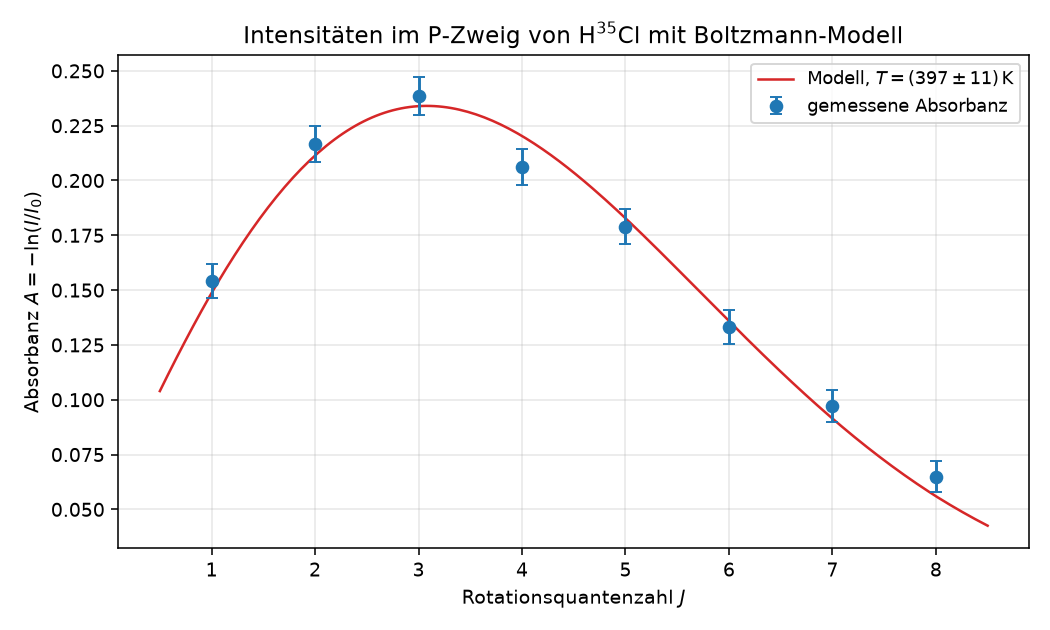
\includegraphics[width=0.72\textwidth]{a6_intensitaet}
  \caption{Gemessene Absorbanzen der P-Zweig-Linien von
    $\mathrm{H}^{35}\mathrm{Cl}$ (Punkte) und angepasstes Boltzmann-Modell nach
    Gl.~\eqref{eq:intmodell} (Linie). Das Intensitätsmaximum bei $J=3$ wird gut
    wiedergegeben.}
  \label{fig:a6_intensitaet}
\end{figure}

Das Modell beschreibt den charakteristischen Intensitätsverlauf mit dem Maximum
bei $J=3$ sehr gut (Abb.~\ref{fig:a6_intensitaet}). Als freier Parameter ergibt
sich die Temperatur
\begin{equation}
  T = (397 \pm 11)\,\si{\kelvin} .
\end{equation}
Der Wert liegt oberhalb der Raumtemperatur von etwa $\SI{300}{\kelvin}$, bei der
die Messung durchgeführt wurde. Diese Überschätzung ist im Wesentlichen darauf
zurückzuführen, dass die intensiven Linien bei kleinen $J$ teilweise gesättigt
sind und ihre Absorbanz dadurch unterschätzt wird; das Intensitätsmaximum
erscheint dadurch zu höheren $J$ verschoben, was im Modell einer höheren
Temperatur entspricht. Innerhalb dieser systematischen Einschränkung gibt der Fit
die Größenordnung der Messtemperatur korrekt wieder und liegt in guter
Übereinstimmung mit vergleichbaren Auswertungen dieses Versuchs.

% ==================================================================
%  4.7  FEHLERBETRACHTUNG
% ==================================================================
\subsection{Fehlerbetrachtung}
\label{sec:fehler}

Im Folgenden werden die Unsicherheiten der bestimmten Größen systematisch
diskutiert. Es wird zwischen statistischen und systematischen Beiträgen
unterschieden und die Gauß'sche Fehlerfortpflanzung angewandt.

\paragraph{Grundlegende Fehlerquellen.}
Alle Wellenzahlen sind mit zwei prinzipiellen Unsicherheiten behaftet:
\begin{itemize}
  \item \emph{Statistische Ableseunsicherheit.} Die spektrale Auflösung der
    HCl-Messung beträgt nach Gl.~\eqref{eq:aufloesung} mit $n=16001$ Punkten und
    $\Delta s=\SI{6.36e-5}{cm}$ etwa $\Delta\bar\nu\approx\SI{0.98}{cm^{-1}}$.
    Unter Annahme einer Rechteckverteilung über eine Auflösungsbreite folgt eine
    Ableseunsicherheit einer Linienposition von
    $\sigma_{\bar\nu}\approx\Delta\bar\nu/\sqrt{12}\approx\SI{0.28}{cm^{-1}}$.
  \item \emph{Systematischer Eichfehler.} Die Kalibrierung (Aufgabe~1.1) liefert
    $\bar\nu_\mathrm{korr}=(\bar\nu_\mathrm{mess}-b)/a$ mit
    $a=1{,}00103\pm0{,}00025$ und $b=(-0{,}47\pm0{,}49)\,\si{cm^{-1}}$. Für eine
    absolute Wellenzahl um $\SI{2887}{cm^{-1}}$ ergibt sich daraus über
    \begin{equation}
      \sigma_{\bar\nu}^\mathrm{eich}
      = \sqrt{\left(\frac{\bar\nu-b}{a^2}\sigma_a\right)^2
             +\left(\frac{\sigma_b}{a}\right)^2}
      \approx \SI{0.87}{cm^{-1}} .
    \end{equation}
\end{itemize}
Entscheidend ist, dass der Eichfehler \emph{korreliert} auf alle Linien wirkt: In
absolute Größen (z.\,B.\ die Bandmitte $\bar\nu_S$) geht er voll ein, während er
sich in \emph{Differenzgrößen} -- und damit in der Rotationskonstante $B$, die aus
Linienabständen folgt -- weitgehend heraushebt. Dort verbleibt lediglich der
multiplikative Skalenfehler $\sigma_a/a\approx2{,}5\cdot10^{-4}$.

\paragraph{Molekülkonstanten (Aufgabe 1.5).}
Die statistischen Unsicherheiten der Fitparameter ergeben sich aus der
Kovarianzmatrix der gewichteten Regression (Gewicht $\sigma_{\bar\nu}$). Die
abgeleiteten Größen folgen mit
\begin{align}
  I = \frac{h}{8\pi^2 c\,B_0} &\Rightarrow \frac{\sigma_I}{I}=\frac{\sigma_{B_0}}{B_0}, &
  r_0 = \sqrt{I/\mu} &\Rightarrow \frac{\sigma_{r_0}}{r_0}=\frac12\frac{\sigma_I}{I}, \\
  k = (2\pi c\,\bar\nu_S)^2\mu &\Rightarrow \frac{\sigma_k}{k}=2\frac{\sigma_{\bar\nu_S}}{\bar\nu_S} .
\end{align}
Für $\bar\nu_S$ dominiert der Eichfehler ($\sigma_\mathrm{stat}\approx\SI{0.12}{cm^{-1}}$
gegenüber $\sigma_\mathrm{eich}\approx\SI{0.87}{cm^{-1}}$), sodass
$\sigma_{\bar\nu_S}\approx\SI{0.88}{cm^{-1}}$. Da $\bar\nu_S$ groß ist, bleibt der
relative Fehler klein und pflanzt sich nur schwach auf $k$ fort. Die vollständig
propagierten Unsicherheiten sind in Tab.~\ref{tab:a5} bereits berücksichtigt; sie
betragen $\sigma_{B_0}\approx\SI{0.02}{cm^{-1}}$, $\sigma_{r_0}\approx\SI{0.15}{pm}$
und $\sigma_k\approx\SI{0.3}{N/m}$. Die Isotopenverhältnisse
$\bar\nu_S(^{35})/\bar\nu_S(^{37})=1{,}00073\pm0{,}00043$ und
$B_0(^{35})/B_0(^{37})=1{,}0013\pm0{,}0033$ sind damit innerhalb ihrer Fehler mit
den theoretischen Werten verträglich.

\paragraph{Temperatur (Aufgabe 1.6).}
Die Absorbanzen $A=-\ln(I/I_0)$ tragen die Unsicherheit
$\sigma_A=\sigma_T/T$, wobei das Basislinienrauschen der Transmission zu
$\sigma_T\approx0{,}007$ bestimmt wurde. Die gewichtete Anpassung des
Boltzmann-Modells liefert $T=(397\pm11)\,\si{\kelvin}$ bei einem reduzierten
$\chi^2/\mathrm{dof}\approx1{,}1$, was auf eine konsistente Fehlerabschätzung
hindeutet. Der Wert enthält jedoch einen nicht in der statistischen Unsicherheit
erfassten \emph{systematischen} Beitrag durch die Sättigung der intensiven Linien
(siehe Aufgabe~1.6), der die Abweichung von der Raumtemperatur erklärt.

\paragraph{Häufigkeitsverhältnis (Aufgabe 1.5).}
Das aus $14$ Dublett-Paaren gemittelte Verhältnis beträgt
$N_{35}/N_{37}=1{,}96\pm0{,}08$ (Standardfehler des Mittelwerts bei einer
Streuung von $\sigma=0{,}31$). Die deutliche Abweichung vom Literaturwert $3{,}13$
ist systematischer Natur (Linien\-sättigung) und nicht durch den statistischen
Fehler abgedeckt.

\paragraph{Spaltbreite (Aufgabe 1.4).}
Der rein statistische Fehler der Regression $N(\bar\nu)$ ist mit
$\sigma_\mathrm{stat}<\SI{0.05}{\micro\metre}$ (einschließlich des Eichbeitrags
$\sigma_a/a$) unrealistisch klein, da er die systematischen Einflüsse der
Untergrund- und Bandpasswahl nicht erfasst. Als realistische Unsicherheit wird
daher die Abweichung zwischen der Peak- und der Fourier-Methode
($\approx\SI{1}{\micro\metre}$) angesetzt. Die verbleibende Differenz der beiden
Küvettenwerte ($47{,}5$ vs.\ $49{,}8\,\si{\micro\metre}$) liegt in derselben
Größenordnung und spiegelt reale Fertigungs- bzw.\ Justageunterschiede wider.

\paragraph{Sperrfilter (Aufgabe 1.3).}
Die Transmissionswerte im Sperrbereich sind Mittelwerte über viele Datenpunkte;
ihr Standardfehler des Mittelwerts ist mit
$(0{,}026\pm0{,}003)\,\si{\percent}$ (Glas) bzw.\
$(0{,}35\pm0{,}06)\,\si{\percent}$ (NaCl) klein. Die größere Streuung bei NaCl
($\sigma\approx1{,}8\,\si{\percent}$) resultiert aus der kleinen
Referenzintensität $I_0$ im ferninfraroten Sperrbereich, wo sich das Rauschen bei
der Division stark auswirkt.

% ==================================================================
%  5  FAZIT
% ==================================================================
\section{Fazit}
\label{sec:fazit}

Mit dem FTIR-Spektrometer Perkin~Elmer~Spectrum~100 wurden verschiedene Proben im
infraroten Spektralbereich untersucht. Die Überprüfung der Wellenzahlskala anhand
der Kalibrierbanden von Wasserdampf und Polystyrol ergab mit einem Anstieg von
$a=1{,}00103 \pm 0{,}00025$ und einem Achsenabschnitt von $(-0{,}47\pm0{,}49)\,
\si{cm^{-1}}$ eine innerhalb der Messgenauigkeit korrekte Kalibrierung. Aus den
Interferogrammen verschiedener Länge wurde die Schrittweite des optischen Weges zu
$\Delta s \approx \SI{6.36e-5}{cm}$ bestimmt und der Einfluss von
Interferogrammlänge, Zerofilling und Apodisation auf die Spektren diskutiert; das
theoretische Auflösungsvermögen reicht von $\SI{15.7}{cm^{-1}}$ (kürzeste Messung)
bis $\SI{0.39}{cm^{-1}}$ (längste Messung). Die Sperrfilter zeigten im jeweiligen
Sperrbereich ein Transmissionsvermögen von deutlich unter $\SI{1}{\percent}$,
wobei Glas das gesamte mittlere Infrarot blockiert und NaCl darin transparent ist.
Die Spaltbreite zweier Küvetten wurde mit der Interferenzmethode zu $(47{,}5\pm
1{,}0)\,\si{\micro\metre}$ bzw.\ $(49{,}8\pm1{,}0)\,\si{\micro\metre}$ bestimmt.

Kernstück war die Analyse des Rotations-Schwingungsspektrums von HCl, aus dem sich
für $\mathrm{H}^{35}\mathrm{Cl}$ eine Schwingungswellenzahl von
$\bar\nu_S=\SI{2888.8}{cm^{-1}}$, eine Rotationskonstante $B_0=\SI{10.45}{cm^{-1}}$,
ein Kernabstand $r_0=\SI{128.3}{pm}$ und eine Kraftkonstante $k=\SI{482}{N/m}$
ergaben -- allesamt in guter Übereinstimmung mit den Literaturwerten. Die
Isotopenaufspaltung und die Verhältnisse der Molekülkonstanten beider Isotopologe
bestätigen die theoretische Massenabhängigkeit. Das Häufigkeitsverhältnis
$N_{35}/N_{37}=1{,}96\pm0{,}08$ und die aus der Intensitätsmodellierung bestimmte
Temperatur $T=(397\pm11)\,\si{\kelvin}$ liegen aufgrund von Sättigungseffekten der
starken Linien etwas neben den Erwartungswerten, geben deren Größenordnung aber
korrekt wieder.

% ==================================================================
%  LITERATUR
% ==================================================================
\newpage
\begin{thebibliography}{9}

\bibitem{Riede}
  V.~Riede (Überarb.\ C.~Kranert):
  \emph{Rotations-Schwingungsspektren von Molekülen},
  Versuchsanleitung zum Fortgeschrittenenpraktikum,
  Universität Leipzig.

\bibitem{Finkelnburg}
  W.~Finkelnburg:
  \emph{Einführung in die Atomphysik},
  Springer-Verlag, Berlin/Göttingen/Heidelberg 1958, S.~186\,ff und S.~351\,ff.

\bibitem{Bruegel}
  W.~Brügel:
  \emph{Einführung in die Ultrarotspektroskopie},
  Dr.\ Dietrich Steinkopff Verlag, Darmstadt 1969, S.~9--27.

\bibitem{Herzberg}
  G.~Herzberg:
  \emph{Molecular Spectra and Molecular Structure},
  Bd.~I (Spectra of Diatomic Molecules),
  D.~van Nostrand Comp., Toronto/New York/London 1950.

\bibitem{Geschke}
  D.~Geschke:
  \emph{Physikalisches Praktikum},
  B.~G.~Teubner, Stuttgart/Leipzig 1994.

\bibitem{Demtroeder}
  W.~Demtröder:
  \emph{Molekülphysik}, 2.~Auflage,
  Oldenbourg Wissenschaftsverlag, Berlin 2013, S.~91.

\bibitem{FTIRhist}
  Universität Leipzig, AG Optik/Spektroskopie:
  \emph{Geschichte der FTIR-Spektroskopie},
  \url{https://polariton.exphysik.uni-leipzig.de/subsites/staff/bundesmann/ftir/geschichte.html}

\bibitem{Rinsland}
  C.~P.~Rinsland et al.:
  \emph{The Fundamental Bands of \textsuperscript{35}HCl and \textsuperscript{37}HCl:
  Line Positions from High-Resolution Laboratory Data},
  Journal of Molecular Spectroscopy, Vol.~159 (1993).

\bibitem{Gupta}
  D.~Gupta, L.~Wang, L.~M.~Hanssen, J.~J.~Hsia, R.~U.~Datla:
  \emph{Polystyrene Films for Calibrating the Wavelength Scale of Infrared
  Spectrophotometers -- SRM~1921},
  NIST Special Publication 260-122 (1995).

\end{thebibliography}

\end{document}
